%%%%%%%%%%%%%%%%%%%%%%%%%%%%%
% Sorry, I don't know how to do it better...
%%%%%%%%%%%%%%%%%%%%%%%%%%%%%
\newcommand\partquatre{%
  \cleardoublepage
  \thispagestyle{plain}%
  \null\vfil
   \secdef\kkkpart\kkkpart}
\def\kkkpart[#1]#2{%
      \relax
      \refstepcounter{part}%
      \addcontentsline{toc}{part}{\thepart\hspace{1em}#1}%
    {\centering
     \interlinepenalty
     \normalfont
      \relax
       \huge\bfseries \partname\nobreakspace\thepart
       \par
       \vskip 20pt
     \Huge \bfseries #2\par}%
    \kkkendpart}
\def\kkkendpart{
\vspace*{3cm}
\begin{center}
\begin{minipage}{0.8\textwidth}
\textbf{ \noindent Fins ara, els vostres programes han executat totes i cada una de les seves expressions. No heu disposat de cap manera d'expressar que algunes parts d'un programa haurien de ser executades només si es compleixen certes condicions. En aquesta part, us presentem les expressions condicionals, que resolen aquest problema. Aquesta part també introdueix la noció de referències en l'espai bidimensional d'un pla i altres comportaments dels robots. Finalment us ensenyarem com utilitzar un robot per simular el comportament d'animals simples.}
\end{minipage}
\end{center}
	\vfil\newpage
                \null
                \thispagestyle{empty}}
%%%%%%%%%%%%%%%%%%%%%%%%%%%%%
%%%%%%%%%%%%%%%%%%%%%%%%%%%%%
%%%%%%%%%%%%%%%%%%%%%%%%%%%%%

\partquatre{Condicionals}

\chapter{Condicions}
\label{cap18}
\index{errors|seealso{depurador; errors de programa}}
Fins ara, els programes que heu definit executen \emph{totes} les expressions que contenen, una darrera l'altra. No teniu cap manera de dir que algunes expressions s'haurien d'executar només si determinades \emph{condicions} es satisfan. Aquest capítol i el següent introdueixen un concepte molt important en programació: la noció d'\emph{execució} condicional, és a dir, l'execució d'un determinat fragment de codi només quan es compleix certa condició. Formalment, una \emph{condició} és una expressió que pot ser o bé cert (\textsf{true}) o bé fals (\textsf{false}).

Aquest capítol comença definint un problema senzill que mostra la necessitat de l'execució condicional. Després veurem que una expressió condicional està composta d'una \emph{condició} i d'un \emph{missatge condicional} que pren un o més arguments, l'execució del qual depèn del valor de la condició. Els arguments d'un missatge condicional s'anomenen \emph{blocs condicionals}, i són seqüències d'expressions tancades entre claudàtors [ ].

\section{Els autèntics colors d'un robot}
\index{colors!canviar-los en els robots|(}
\index{robots!canviar colors|(}
\index{expressions condicionals!utilitzar per canviar els colors d'un robot|(}
Imaginem que volem canviar el color d'un robot depenent de la seva distància al centre de la pantalla. Si un robot és a menys de 200 píxels del centre, hauria de ser vermell. Sinó, hauria de ser verd. Aquest problema requereix una execució \emph{condicional}. En funció d'una condició --la posició del robot-- el color hauria de canviar.

El mètode \textsf{detectorDistancia}, que podeu veure com a Mètode~\ref{met18-1}, mostra una possible solució, i l'\emph{Script}~\ref{scr18-1} us ensenya com s'ha d'utilitzar.
\begin{script}  Pica canvia el color d'acord amb el mètode \textsf{\upshape detectorDistancia}.
\textsf{\upshape
\begin{tabbing}
\hspace{5mm} \= \kill
$|$ pica $|$\\
pica := Bot nou.\\
pica salta: 20.\\
pica detectorDistancia.\\
pica salta: 200.\\
pica detectorDistancia.
\end{tabbing}}
\label{scr18-1}
\end{script}
\begin{metode} Instruccions per tal que qualsevol robot dibuixi un quadrat senzill.
\noindent
\textsf{\upshape
\begin{tabbing}
\hspace{5mm} \= \hspace{10mm} \= \kill
{\bfseries detectorDistancia}\\
\\
\> $|$ distanciaDelCentre $|$\\
\> distanciaDelCentre := self distanciaDesde: World center.\\
\> distanciaDelCentre \textless \hspace*{1mm}   200\\
\>\> siCert: [  self color: Color vermell  ]\\
\>\> siFals: [  self color: Color verd  ]
\end{tabbing}
}
\label{met18-1}
\end{metode}
Analitzem què passa quan l'expressió \textsf{pica detectorDistancia} s'executa. Primer, l'expressió \textsf{self distanciaDesde: World center} calcula la distància del receptor al centre de la pantalla. Aquesta distància és guardada a la variable \textsf{distanciaDelCentre}. \index{detectorDistancia mètode!canviar els colors amb}

Després l'expressió \textsf{distanciaDelCentre \textless \hspace*{1mm}   200 siCert: [  self color: Color vermell  ] siFals: [  self color: Color verd  ]}
s'executa de la següent manera: \emph{si} la distància del centre és inferior a 200, el color del receptor és canviat a vermell; sinó, és canviat a verd. Aquesta expressió és una expressió \emph{condicional}. Ocupa tres línies dins la definició del mètode, però és una sola expressió, i la podeu distingir ja que no hi ha cap punt entre cap de les seves parts.

Diguem-ho un altre cop, una expressió condicional es compon de dues parts: una \emph{condició} i un \emph{missatge condicional} els arguments del qual són \emph{blocs condicionals}. L'expressió \textsf{distanciaDelCentre \textless \hspace*{1mm}   200} és una condició, l'expressió  \textsf{siCert: [  self color: Color vermell  ] siFals: [  self color: Color verd  ]} és un missatge condicional, i  \textsf{[  self color: Color vermell  ]} i \textsf{[  self color: Color verd  ]} són blocs condicionals, com podeu veure a la figura~\ref{fig1801}.
\begin{figure}[h!]
\begin{center}
\includegraphics[scale=0.7]{Imatges/figura18-1.pdf}
\end{center}
\caption{Una expressió condicional es compon d'una condició i d'un missatge condicional, els arguments del qual són blocs condicionals.}
\label{fig1801}
\end{figure}

El mètode \textsf{siCert:siFals:}\footnote{\emph{Nota del Traductor:} Tal com hem explicat al principi del llibre, aquest mètode està traduït. L'original Smalltalk és \textsf{ifTrue:ifFalse:}.} executa una condició, aquí \textsf{distanciaDelCentre \textless \hspace*{1mm}   200}, i en funció del seu valor, executa un dels blocs condicionals i no executa l'altre. La paraula clau \textsf{siCert:} indica que el bloc condicional \textsf{[ self color: Color vermell ]} s'executa només si la condició és certa. Igualment, la paraula clau \textsf{siFals:} indica que el bloc condicional \textsf{[ self color: Color verd ]} s'executa només si la condició és falsa. Els blocs condicionals també s'anomenen bifurcacions de la condició. Suposeu que esteu resseguint amb el dit, en una fotografia, el tronc d'un arbre, i cada cop que trobeu una branca heu de decidir quin camí seguir, i només podeu seguir un camí a la vegada. El terme \emph{bifurcació} es refereix a aquesta situació. Representa el fet que l'execució del programa ha de triar entre camins i executar només un camí, prescindint de l'altre camí.\index{siCert:siFals: mètode!efecte de}

Ja heu vist dos tipus diferents d'expressió: un tipus, per exemple \textsf{self distanciaDesde: World center}, s'executa sempre que la trobem en un programa, mentre que l'altre tipus, aquelles que estan dins de blocs condicionals, s'executen només quan la condició associada és certa o falsa, depèn de quin sigui el cas.

Un bloc condicional no està limitat a una sola expressió, sinó que pot contenir una seqüència d'expressions, com veurem al proper capítol. Així, el mètode \textsf{siCert:siFals:} defineix dos blocs condicionals, cada un contenint una \emph{seqüència} d'expressions (com veureu a la propera secció, fins i tot podeu tenir una seqüència de cap expressió).

Finalment, fixeu-vos que el mètode \textsf{siCert:siFals:} és \emph{un} mètode amb \emph{dos} arguments, un pel cas cert i l'altre pel cas fals. Per tant no heu de posar cap punt després del claudàtor dret ] que tanca el bloc \textsf{siCert:}, ja que trencaríeu la instrucció condicional acabant-la massa aviat, i provocaríeu un error. \index{robots!canviar colors|)}

\subsection{Afegir una traça per veure què va passant}
\index{expressions condicionals!utilitzar per canviar els colors d'un robot|)}
\index{expressions condicionals!utilitzar traces amb|(}
\index{traces!utilitzar en expressions condicionals|(}
\index{Transcript@\emph{Transcript}, eina!utilitzar en expressions condicionals|(}
Per entendre com s'executen les expressions condicionals, hauríeu d'experimentar enviant missatges al \textsf{Transcript} per generar una traça, com vam veure al capítol~\ref{cap17}. També podeu utilitzar el depurador inserint l'expressió \textsf{self halt}, com us vam ensenyar al capítol~\ref{cap15}. Si voleu saber si s'està executant algun dels blocs condicionals en particular, introduïu expressions en aquell bloc. Per exemple, podríeu inserir l'expressió \textsf{Transcript show: 'ara executant el bloc corresponent a cert' ; cr } a la branca \textsf{siCert:}. El Mètode~\ref{met18-2} presenta una manera de generar una traça com la mencionada al context del mètode \textsf{detectorDistancia}. Depenent de la posició del robot, es generaran traces diferents. Proveu d'endevinar les traces abans d'executar l'\emph{Script}~\ref{scr18-1}. No dubteu a afegir i modificar aquest tipus de traces a tots els \emph{scripts} que trobeu difícils d'entendre.\index{detectorDistancia mètode!amb una traça}
\begin{metode} El mètode per detectar la distància amb una traça.
\noindent
\textsf{\upshape
\begin{tabbing}
\hspace{5mm} \= \hspace{10mm} \= \kill
{\bfseries detectorDistancia}\\
\> $|$ distanciaDelCentre $|$\\
\> distanciaDelCentre := self distanciaDesde: World center.\\
\> {\bfseries Transcript show: 'sempre' ; cr }.\\
\> distanciaDelCentre \textless \hspace*{1mm}   200\\
\>\> siCert: [ \= self color: Color vermell.\\
\>\>\> {\bfseries Transcript show: 'vermell' ; cr }  ]\\
\>\> siFals: [  self color: Color verd.\\
\>\>\> {\bfseries Transcript show: 'verd' ; cr }  ]
\end{tabbing}
}
\label{met18-2}
\end{metode}

\subsection{El valor retornat per un mètode}
\index{valors!retornat pels mètodes}
\index{metodes@mètodes!valor retornat per}
\index{colors!canviar-los en els robots|)}
\index{bloc condicional, exemple de}
\index{expressions condicionals!utilitzar traces amb|)}
\index{traces!utilitzar en expressions condicionals|)}
\index{Transcript@\emph{Transcript}, eina!utilitzar en expressions condicionals|)}
Quan us vam ensenyar com definir mètodes al capítol~\ref{cap12}, vam explicar que executant un mètode no només s'avaluen els missatges que conté, sinó que a més \emph{retorna} un valor. Fins ara, no hem posat especial èmfasi en els valors retornats pels mètodes. Ara, però, començarem a fixar-nos en els valors retornats per la condició d'una expressió condicional. Per exemple, la condició \textsf{distanciaDelCentre \textless \hspace*{1mm}   200} retorna un valor (cert o fals) que ens diu si la distància al centre de la pantalla és o no és inferior a 200 (aprendreu més sobre \textsf{true} --cert-- i \textsf{false} --fals-- al capítol~\ref{cap20}).

Altres expressions que apareixen al Mètode~\ref{met18-1} retornen valors d'interès. Per exemple, no només l'expressió \textsf{self distanciaDesde: World center} calcula la distància del receptor al centre de la pantalla, sinó que també \emph{retorna} aquesta distància. Després, la condició  \textsf{distanciaDelCentre \textless \hspace*{1mm}   200} utilitza aquesta distància per decidir quina branca de l'expressió condicional hauria de ser executada.\index{[] (claudàtors)!utilitzar en blocs condicionals} \index{claudàtors ([])!utilitzar en blocs condicionals}

\noindent
\rule{\textwidth}{2pt}
\noindent
\textbf{Important!} Una expressió condicional es compon d'una \emph{condició} i d'un \emph{missatge condicional} que pren un o més arguments i l'execució del qual depèn del valor d'una condició. Els arguments d'un missatge condicional s'anomenen \emph{blocs condicionals}, i són seqüències d'expressions tancades entre claudàtors [ ]:\index{expressions condicionals!components de}
\noindent
\textsf{\upshape
\begin{tabbing}
\hspace{10mm} \= \kill
{\itshape unaCondicio}\\
\> {\bfseries siCert:  [  } {\itshape expressionsSiCondicioEsCerta }{\bfseries  ] }\\
\> {\bfseries siFals:  [  } {\itshape expressionsSiCondicioEsFalsa }{\bfseries  ] }
\end{tabbing}}
\noindent
\rule{\textwidth}{2pt}

\section{Expressions condicionals amb una sola bifurcació}
\index{expressions condicionals!amb una sola bifurcació|(}
\index{siFals: mètode, efecte de|(}
\index{siCert:siFals: mètode!utilitzar bloc condicional buit amb}
Algunes vegades, heu de realitzar una acció quan determinada condició és certa, però si la condició és falsa no voleu fer res (i viceversa). Prenent un exemple de la vida real, si porteu un paraigües tancat i comença a ploure, voleu obrir-lo, però si no plou, no voleu fer res de res. Prenent un exemple d'Squeak, el mètode \textsf{vermellSiPropDelCentre} (Mètode~\ref{met18-3}) canvia el color del receptor a vermell quan és a una distància més petita que 200 píxels del centre de la pantalla, però si la distància no és més petita que 200 píxels, el color del robot no canvia.
\begin{metode} Si voleu no fer res quan la condició és falsa, podeu utilitzar un bloc condicional buit amb \textsf{\upshape siCert:siFals:}.
\noindent
\textsf{\upshape
\begin{tabbing}
\hspace{5mm} \= \hspace{10mm} \= \kill
{\bfseries vermellSiPropDelCentre}\\
\\
\> $|$ distanciaDelCentre $|$\\
\> distanciaDelCentre := self distanciaDesde: World center.\\
\> distanciaDelCentre \textless \hspace*{1mm}   200\\
\>\> {\bfseries siCert:} [  self color: Color vermell  ]\\
\>\> {\bfseries siFals:} [   ]
\end{tabbing}
}
\label{met18-3}
\end{metode}

Amb el mètode \textsf{siCert:siFals:}, deixeu la segona branca buida, amb un bloc condicional sense cap expressió: [ ]. Smalltalk, però, proporciona dos mètodes alternatius, \textsf{siCert:} i \textsf{siFals:}, per escriure aquesta classe d'expressions condicionals. El mètode \textsf{siCert:} executa el seu bloc condicional quan la condició és certa. Utilitzant el mètode \textsf{siCert:} podem reescriure el Mètode~\ref{met18-3} més convenientment com el Mètode~\ref{met18-4}.
\begin{metode} Amb el mètode \textsf{\upshape siCert:}, ja no us cal un bloc condicional buit.
\noindent
\textsf{\upshape
\begin{tabbing}
\hspace{5mm} \= \hspace{10mm} \= \kill
{\bfseries vermellSiPropDelCentre}\\
\\
\> $|$ distanciaDelCentre $|$\\
\> distanciaDelCentre := self distanciaDesde: World center.\\
\> distanciaDelCentre \textless \hspace*{1mm}   200\\
\>\> {\bfseries siCert:} [  self color: Color vermell  ]\\
\end{tabbing}
}
\label{met18-4}
\end{metode}

El mètode \textsf{siFals:} és completament anàleg al mètode \textsf{siCert:}, executa el seu bloc condicional quan la condició és \emph{falsa}. Cada un dels mètodes \textsf{siCert:} i \textsf{siFals:} executa una condició i després, en funció del valor retornat per la condició, el mètode executa, o no, el bloc condicional.
\newpage
\noindent
\rule{\textwidth}{2pt}
\noindent
\textbf{Important!} El mètode \textsf{siCert:} executa el seu bloc condicional quan la condició és certa. El mètode \textsf{siFals:} executa el seu bloc condicional quan la condició és falsa.
\noindent
\textsf{\upshape
\begin{tabbing}
\hspace{10mm} \= \kill
{\itshape unaCondicio}\\
\> {\bfseries siCert:  [  } {\itshape expressionsSiCondicioEsCerta }{\bfseries  ] }\\
{\itshape unaCondicio}\\
\> {\bfseries siFals:  [  } {\itshape expressionsSiCondicioEsFalsa }{\bfseries  ] }
\end{tabbing}}
\noindent
\rule{\textwidth}{2pt}

\subsection{Triar el mètode condicional adequat}
\index{condicionals mètodes, triar}
Utilitzar \textsf{siCert:siFals:} no és el mateix que utilitzar \textsf{siCert:} seguit de \textsf{siFals:}. Amb  \textsf{siCert:siFals:} la condició que el precedeix només s'executa una vegada, però si voleu utilitzar \textsf{siCert:} seguit de \textsf{siFals:}, us cal una condició davant de cada missatge, i totes dues seran executades, fins i tot si són idèntiques. Això pot donar lloc a conseqüències no desitjades si el bloc condicional de la primera expressió condicional (\textsf{siCert:}) modifica allò que comprovem a la condició de la segona expressió condicional  (\textsf{siFals:}). En aquest cas, utilitzar \textsf{siCert:} seguit de \textsf{siFals:} no és equivalent a utilitzar \textsf{siCert:siFals:}.

\section{Imbricar expressions condicionals}
\index{expressions condicionals!imbricar|(}
\index{siFals: mètode, efecte de|)}
\index{expressions condicionals!amb una sola bifurcació|)}
Una expressió condicional pot contenir qualsevol altra expressió dins dels seus blocs condicionals, en particular, aquests blocs poden contenir altres expressions condicionals. Això és el que ara tractarem. No hi ha res conceptualment nou, però és una pràctica útil i habitual, per tant pensem que és interessant que us l'ensenyem.

\subsection{Acolorir robots amb tres colors}
\index{colors!canviar-los en els robots|(}
\index{robots!acolorir|(}
Modifiquem el problema anterior. Si un robot és a menys de 200 píxels del centre de la pantalla, hauria de ser de color vermell; si està situat entre 200 i 300 píxels lluny del centre, hauria de ser de color groc, i si la distància és superior a 300 píxels, hauria de ser de color verd.

En aquest problema, diferents parts del mètode haurien de ser executades sota circumstàncies diferents. És a dir, hi ha tres rangs diferents de distàncies, i el color del robot hauria de canviar a vermell, groc o verd depenent d'on es trobi. Una solució possible al nostre problema la podem veure al Mètode~\ref{met18-5}. El que hem fet és dividir el problema en dos trossos: què fer si la distància del robot al centre és superior a 300 píxels, i què fer si no ho és. Després dividim el tros ``què fer si no'' en dos subproblemes: què fer si la distància al centre és inferior a 200, i què fer si no ho és.
\begin{metode} Acolorim el robot amb un color, entre tres colors possibles, en funció de la seva distància del centre de la pantalla.
\noindent
\textsf{\upshape
\begin{tabbing}
\hspace{5mm} \= \hspace{5mm} \= \kill
{\bfseries modificaTresColors}\\
\\
\> $|$ distancia $|$\\
\> distancia := self distanciaDesde: World center.\\
\> distancia \textgreater \hspace*{1mm}   300\\
\>\> siCert: [  self color: Color verd  ]\\
\>\>  siFals: [  \= distancia \textless \hspace*{1mm}  200\\
\>\>\>  siCert: [  self color: Color vermell  ]\\
\>\>\>  siFals: [  self color: Color groc  ]  ]
\end{tabbing}
}
\label{met18-5}
\end{metode}

El Mètode~\ref{met18-6} conté exactament el mateix codi, amb codi emfatitzat per mostrar les expressions condicionals. Hi ha dues expressions condicionals diferents. La primera (Expressió condicional 1) es mostra en itàlica, i la segona (Expressió condicional 2) en negreta. La segona expressió condicional s'executa només si la condició de la primera expressió condicional és falsa. És a dir, si la distància és menor o igual a 200, aleshores l'expressió condicional 2 s'executa. Si l'expressió condicional 2 s'executa, la seva condició \textsf{distancia \textless \hspace*{1mm}   200} també s'executa, i en funció del seu valor, la branca \textsf{siCert:} o la branca \textsf{siFals} s'executaran. Aquí teniu les dues expressions condicionals:

\vspace*{3mm}
\noindent
{\bf \large Expressió condicional 1:}
%\vspace*{1mm}
\noindent
\textsf{\upshape
\begin{tabbing}
\hspace{5mm} \= \kill
{\itshape distancia \textgreater \hspace*{1mm}   300}\\
\> {\itshape siCert: [  self color: Color verd  ]}\\
\> {\itshape siFals: [  ``executa l'expressió condicional 2''  ]}\\
\end{tabbing}}

\noindent
{\bf \large Expressió condicional 2:}
%\vspace*{1mm}
\noindent
\textsf{\upshape
\begin{tabbing}
\hspace{5mm} \= \kill
{\bfseries distancia \textless \hspace*{1mm}    200}\\
\> {\bfseries siCert: [  self color: Color vermell  ]}\\
\> {\bfseries siFals: [  self color: Color groc  ]}\\
\end{tabbing}}

\noindent
I aquí teniu el Mètode~\ref{met18-6}.
\newpage
\begin{metode} Aquest és el Mètode~\ref{met18-5} emfatitzat.
\noindent
\textsf{\upshape
\begin{tabbing}
\hspace{5mm} \= \hspace{5mm} \= \kill
{\bfseries modificaTresColors}\\
\\
\> $|$ distancia $|$\\
\> distancia := self distanciaDesde: World center.\\
\> distancia \textgreater \hspace*{1mm}   300\\
\>\> {\itshape siCert: [  self color: Color verd  ]}\\
\>\> {\itshape siFals: [}  \= {\itshape distancia \textless \hspace*{1mm}  200}\\
\>\>\> {\bfseries siCert: [  self color: Color vermell  ]}\\
\>\>\> {\bfseries siFals: [  self color: Color groc  ] ]}
\end{tabbing}}
\label{met18-6}
\end{metode}

Si teniu dificultats identificant quin bloc condicional serà executat, trieu alguns valors particulars per a la distància (com per exemple, 150, 250 i 350). Proveu de fer una execució manual del mètode i subratlleu la part del mètode que serà executada. Seguint cada pas veureu que només s'executen algunes branques. Podeu afegir algunes traces per mostrar com s'executen les diferents condicions, o podeu utilitzar el depurador per anar executant el mètode pas a pas. \index{colors!canviar-los en els robots|)} \index{robots!acolorir|)}

\section{Aprendre dels errors}
\index{girDeColors: mètode!definir}
\index{colors!relació amb la direcció del robot|(}
\index{expressions condicionals!imbricar|)}
\index{errors!aprendre de|(}
Tothom comet errors. Precisament per això estudiar errors de programació és una manera excel·lent d'aprendre i entendre un concepte des d'una altra perspectiva. Hem definit un mètode \textsf{girDeColors: unAngle} que canvia el color d'un robot  en funció de la direcció a què apunta. Quan el robot apunta al nord, ens agradaria que fos de color blau per representar el fred. Voldríem que fos vermell quan apunta al sud, i en els altres casos, hauria de ser verd. El primer intent de definir aquest mètode, que no va tenir gaire èxit, el teniu com a Mètode~\ref{met18-7}.

\begin{metode} El color del robot depèn de la seva direcció: primer intent (amb un error).
\noindent
\textsf{\upshape
\begin{tabbing}
\hspace{5mm} \= \hspace{5mm} \= \kill
{\bfseries girDeColors: unAngle}\\
\> ``canvia el color del robot de manera que és blau quan apunta al nord,\\
\> vermell si apunta al sud, i verd en els altres casos''\\
\\
\> self gira: unAngle.\\
\> self direccio = 90\\
\>\> siCert: [  self color: Color blau  ].\\
\> self direccio = -90\\
\>\> siCert: [  self color: Color vermell  ]\\
\>\> siFals: [  self color: Color verd  ]
\end{tabbing}
}
\label{met18-7}
\end{metode}

La definició del Mètode~\ref{met18-7} no és correcte. Proveu d'entendre per què no ho és abans de continuar llegint. Seguiu la definició del mètode per veure que quan un robot està apuntant al nord, primer tindrà el color blau, tal com hauríem esperat, però després es tornarà verd, i això no és el que hauria de passar. Hauria de mantenir el color blau després d'haver-li assignat el color blau. L'\emph{Script}~\ref{scr18-2} il·lustra l'error en el mètode. \index{girDeColors: mètode!depurar|(}
\begin{script}  Hi ha un error en el mètode!
\textsf{\upshape
\begin{tabbing}
\hspace{5mm} \= \hspace{70mm} \= \kill
$|$ pica $|$\\
pica := Bot nou.\\
pica girDeColors: -90.\\
pica color.\\
{\itshape -- Escriure el valor retornat: Color red} \>\> {\itshape ``ok''}\\
pica girDeColors: 90.\\
pica color.\\
{\itshape -- Escriure el valor retornat: Color green} \>\> {\itshape ``ok''}\\
pica girDeColors: 90.\\
pica color.\\
-- Escriure el valor retornat: Color green \>\> ``error''\\
\end{tabbing}}
\label{scr18-2}
\end{script}

\emph{Què ha anat malament?} Executeu el Mètode~\ref{met18-7} mentalment per identificar l'error. El problema és que quan el robot està apuntant al nord, la condició \textsf{self direccio = 90} és certa, i el bloc associat s'executa, acolorint el robot de blau. El mètode hauria d'acabar aquí. Però quan el mètode continua i executa el bloc condicional de la segona expressió condicional, el color del robot canvia a verd ja que la direcció del robot no és \textsf{sud}. El següent codi comentat ho il·lustra.

\noindent
\textsf{\upshape
\begin{tabbing}
\hspace{10mm} \= \hspace{5mm} \= \hspace{70mm} \= \kill
pica girDeColors: 90.\\
\\
\> self direccio = 90 \>\>``és cert''\\
\>\> siCert: [ self color: Color blau ] \> ``així el missatge condicional cert \\
\>\>\> s'executa; el robot es torna blau\\
\>\>\>  i avalua la propera condició''\\
\> self direccio = -90 \>\>``és fals''\\
\>\> {\bfseries siFals: [ self color: Color verd ]} \> ``de manera que el missatge condicional\\
\>\>\> fals s'executa. Error!''\\
\end{tabbing}}

\emph{Com corregir-ho?} En fer la traça del mètode, vau veure que quan el robot apunta al nord, la segona expressió condicional no s'hauria d'executar. S'hauria d'executar només si la primera condició és falsa. Per tant, podeu utilitzar expressions condicionals imbricades. El codi correcte el teniu al Mètode~\ref{met18-8}. \index{girDeColors: mètode!depurar|)} \index{colors!relació amb la direcció del robot|)} \index{errors!aprendre de|)}

\begin{metode} El color del robot depèn de la seva direcció: versió correcta.
\noindent
\textsf{\upshape
\begin{tabbing}
\hspace{5mm} \= \hspace{5mm} \= \kill
{\bfseries girDeColors: unAngle}\\
\> ``canvia el color del robot de manera que és blau quan apunta al nord,\\
\> vermell si apunta al sud, i verd en els altres casos''\\
\\
\> self gira: unAngle.\\
\> self direccio = 90\\
\>\> siCert: [  self color: Color blau  ].\\
\>\> siFals: [  self \= direccio = -90\\
\>\>\> siCert: [  self color: Color vermell  ]\\
\>\>\> siFals: [  self color: Color verd  ]  ]
\end{tabbing}
}
\label{met18-8}
\end{metode}

\section{Interpretar un petit llenguatge}
\index{interpretar un petit llenguatge}
\index{llenguatge petit, interpretar|(}
Investigadors en biologia teòrica han desenvolupat sistemes per estudiar el creixement de les plantes, anomenats \emph{Lindenmeyer Systems}. Els sistemes de Lindenmeyer es basen en gràfics de robots semblants als robots amb què ja heu estat experimentant. Els robots de Lindenmeyer entenen un petit llenguatge format per caràcters com \textsf{\$v} i \textsf{\$g}. L'acció d'un robot s'associa a cada un d'aquests caràcters. Per exemple, el caràcter \textsf{\$v} (de ``ves'') és associat al moviment cap a endavant, mentre \textsf{\$g} (de ``gira'') és associat a girar un angle de 45 graus. Un sistema de Lindenmeyer genera una seqüència de caràcters. Aquests caràcters són interpretats per un robot, i la seqüència d'accions que fa el robot genera el dibuix. \index{Lindenmeyer sistemes, significat de}

Anem a definir un mètode \textsf{interpreta: unCaracter} que fa que un robot es mogui endavant si el caràcter és \textsf{\$v} i gira 45 graus en sentit contrari a les agulles del rellotge si el caràcter és \textsf{\$g}. L'\emph{Script}~\ref{scr18-3} il·lustra com utilitzar el mètode, i el mètode es defineix al Mètode~\ref{met18-9}. \index{interpreta: mètode, definir}

\begin{script}  Utilitzar el mètode \textsf{\upshape interpreta: unCaracter}
\textsf{\upshape
\begin{tabbing}
\hspace{5mm} \= \hspace{3mm} \= \kill
$|$ pica $|$\\
pica := Bot nou.\\
4 vegadesRepetir:\\
\> [  pica\\
\>\> interpreta: \$v ; \\
\>\> interpreta: \$g ; \\
\>\> interpreta: \$v ; \\
\>\> interpreta: \$v ; \\
\>\> interpreta: \$g ; \\
\>\> interpreta: \$v  ]
\end{tabbing}}
\label{scr18-3}
\end{script}

\begin{metode} Interpretar un caràcter.
\noindent
\textsf{\upshape
\begin{tabbing}
\hspace{5mm} \= \hspace{5mm} \= \kill
{\bfseries interpreta: unCaracter}\\
\\
\> unCaracter = \$v\\
\>\> siCert: [ self ves: 20 ]\\
\>\> siFals: [\= unCaracter = \$g\\
\>\>\> siCert: [  self gira: 45  ]  ]
\end{tabbing}
}
\label{met18-9}
\end{metode}

Proveu d'escriure un \emph{script} que reprodueixi la figura~\ref{fig1802}. Com que una cadena és una seqüència de caràcters, pot codificar un dibuix generat per un robot de Lindenmeyer. Encara que utilitza uns mètodes que encara no hem explicat (seran explicats a la seqüela d'aquest llibre), intenteu l'\emph{Script}~\ref{scr18-4}, que repetidament envia el missatge \textsf{interpreta:} al robot amb cada caràcter de la cadena. Després, experimenteu una mica més canviant la cadena utilitzada a l'\emph{script} per crear les vostres figures. Construireu un sistema de Lindenmeyer complet a la seqüela d'aquest llibre.
\begin{figure}[h!]
\begin{center}
\includegraphics[scale=1]{Imatges/figura18-2.png}
\end{center}
\caption{Un dibuix generat amb el mètode \textsf{\upshape interpreta:} amb la seqüència de caràcters \textsf{\upshape 'vggvggvggggggvggggggvggvggvggggggvggggggv'}.}
\label{fig1802}
\end{figure}
\newpage
\begin{script}  Utilitzar \textsf{\upshape interpreta:} en un bucle
\textsf{\upshape
\begin{tabbing}
\hspace{5mm} \= \hspace{3mm} \= \kill
$|$ pica $|$\\
pica := Bot nou.\\
'vggvggvggggggvggggggvggvggvggggggvggggggv'\\
\> do: [ :unCaracter | pica interpreta: unCaracter ]
\end{tabbing}}
\label{scr18-4}
\end{script}

\subsection{Més experiments}
Milloreu el mètode \textsf{interpreta: unCaracter} de manera que tant \textsf{\$v} com \textsf{\$V} facin que el robot vagi endavant, i tant \textsf{\$g} com \textsf{\$G} facin que el robot giri 45 graus en sentit contrari a les agulles del rellotge. També podeu utilitzar el caràcter \textsf{\$+} abans de \textsf{\$g} o \textsf{\$G} per fer girar el robot 45 graus en sentit contrari a les agulles del rellotge, i de manera similar \textsf{\$-} per fer-lo girar 45 graus en el sentit de les agulles del rellotge.\index{llenguatge petit, interpretar|)}
\newpage
\section{Resum}
\index{unaCondició (mètode), descripció i exemple de}
Una expressió condicional es compon de dues parts: una \emph{condició} i un \emph{missatge condicional}, que conté un o més \emph{blocs condicionals}. Quin bloc condicional serà executat depèn del valor de la condició. La taula següent mostra alguns dels mètodes utilitzats amb condicions.

\vspace*{2mm}
\noindent
{\footnotesize \begin{tabular}{|l|lllll|}
\rotatebox{90}{\textbf{Exemple}} & 
\rotatebox{90}{
\begin{minipage}{41mm}
\textsf{self direccio = 90} \\ \hspace*{1mm} \textsf{siCert: [ self color: Color verd ]}
\end{minipage}
} & 
\rotatebox{90}{
\begin{minipage}{40mm}
Si un robot apunta al nord, es torna \textsf{verd}.
\end{minipage}
} &
\rotatebox{90}{
\begin{minipage}{40mm}
\textsf{self direccio = 90} \\ \hspace*{1mm} \textsf{siFals: [ Beeper beep ]}
\end{minipage}
} & 
\rotatebox{90}{
\begin{minipage}{40mm}
El sistema es queixa només quan el robot no està apuntant al nord
\end{minipage}
} &
\rotatebox{90}{
\begin{minipage}{41mm}
\textsf{self direccio = 90} \\ \hspace*{1mm} \textsf{siCert: [ self color: Color verd ]} \\ \hspace*{1mm} \textsf{siFals: [ Beeper beep ]}
\end{minipage}
}  \\
\rotatebox{90}{\textbf{Descripció}} & 
\rotatebox{90}{
\begin{minipage}{50mm}
Executa \textsf{\itshape expressionsSiCondicioCerta} només si \textsf{unaCondicio} és certa.
\end{minipage}
} & &
\rotatebox{90}{
\begin{minipage}{50mm}
Executa \textsf{\itshape expressionsSiCondicioFalsa} només si \textsf{unaCondicio} és falsa.
\end{minipage}
} & &
\rotatebox{90}{
\begin{minipage}{50mm}
Executa \textsf{\itshape expressionsSiCondicioCerta} si \textsf{unaCondicio} és certa; en altre cas,
executa \textsf{\itshape expressionsSiCondicioFalsa}.
\end{minipage}
}  \\
\rotatebox{90}{\textbf{Mètode}} & 
\rotatebox{90}{
\begin{minipage}{50mm}
\textsf{{\itshape unaCondicio} \\ \hspace*{1mm} {\itshape siCert: [ expressionsSiCondicioCerta ]}}
\end{minipage}
} & &
\rotatebox{90}{
\begin{minipage}{50mm}
\textsf{{\itshape unaCondicio} \\ \hspace*{1mm} {\itshape siFals: [ expressionsSiCondicioFalsa ]}}
\end{minipage}
} & &
\rotatebox{90}{
\begin{minipage}{50mm}
\textsf{{\itshape unaCondicio} \\ \hspace*{1mm} {\itshape siCert: [ expressionsSiCondicioCerta ]} \\ \hspace*{1mm} {\itshape siFals: [ expressionsSiCondicioFalsa ]}}
\end{minipage}
} 
\end{tabular}}

\chapter{Repeticions condicionals}
\label{cap19}

Les expressions condicionals són una eina molt potent per crear programes complexos ja que us permeten controlar el flux d'execució, bifurcant-lo d'una manera si una determinada condició és certa i d'una altra manera si és falsa. Tot i així, no n'hi ha prou només amb les condicions. Alguns programes necessiten combinar bucles i condicions en \emph{repeticions condicionals}, és a dir, bucles que executen un bloc d'expressions \emph{mentre} es satisfà una determinada condició, aturant l'execució quan aquesta condició ja no es compleix. Aquest capítol presenta els bucles condicionals oferits per Smalltalk i introdueix alguns exemples senzills. Després, al capítol~\ref{cap23}, utilitzarem els bucles condicionals per simular alguns comportaments animals.

\section{Repeticions condicionals}
\index{repeticions condicionals!exemple de|(}
\index{mentreCert: bucle!efecte de} \index{mentreFals: bucle!efecte de}
La idea darrera dels bucles condicionals és que un bloc (una seqüència d'expressions) és repetit mentre es compleixi una certa condició (o, de manera alternativa, mentre una determinada condició no es compleixi). Smalltalk defineix dos missatges, \textsf{whileTrue:} i \textsf{whileFalse:}\footnote{\emph{Nota del Traductor:} Que, com ja hem dit, aquí hem traduït per \textsf{mentreCert:} i \textsf{mentreFals:}.}, que us permeten definir bucles condicionals.

El que fan aquests bucles és clar a partir del nom del mètode: \textsf{mentreCert:} executa la seva condició i executa el bloc condicional mentre la condició sigui certa. El mètode \textsf{mentreFals:} fa el mateix, però executa el bloc condicional només mentre la condició sigui falsa.

\noindent
\rule{\textwidth}{2pt}
\noindent
\textbf{Important!} \textsf{mentreCert:} i \textsf{mentreFals:} us permeten definir bucles condicionals pels que es repeteix el bloc condicional mentre la condició es satisfà (\textsf{mentreCert:}) o no es satisfà (\textsf{mentreFals:})
\noindent
\rule{\textwidth}{2pt}

\subsection{Un exemple}
\index{bucles condicionals|see{repeticions condicionals}}
\index{repeticions condicionals!components de|(}
Anem a posar un exemple senzill. Suposem que tenim un robot en algun lloc a la part sud de la pantalla, on la coordenada \emph{y} és més gran que 100 (per Squeak, l'eix \emph{y} va de nord a sud, és a dir, creix cap avall), i volem que el robot es mogui cap al nord fins que la seva coordenada \emph{y} sigui menor que 100 píxels (veure figura~\ref{fig1901}. Una solució utilitzant un bucle condicional es pot veure al Mètode~\ref{met19-1}, i la podeu fer servir com veieu a l'\emph{Script}~\ref{scr19-1}. \index{finsA100 mètode!efecte de}

\begin{figure}[h!]
\begin{center}
\includegraphics[scale=0.5]{Imatges/figura19-1.pdf}
\end{center}
\caption{El mètode \textsf{\upshape finsA100} mou el robot cap al nord mentre la seva coordenada \emph{y} sigui més gran que 100.}
\label{fig1901}
\end{figure}

\begin{script}  Utilitzar el mètode \textsf{\upshape finsA100}
\textsf{\upshape
\begin{tabbing}
\hspace{5mm} \= \hspace{70mm} \= \kill
$|$ pica $|$\\
pica := Bot nou.\\
pica finsA100
\end{tabbing}}
\label{scr19-1}
\end{script}

\begin{metode} Moure el robot cap al nord mentre la seva coordenada \emph{y} sigui més gran que 100
\noindent
\textsf{\upshape
\begin{tabbing}
\hspace{5mm} \= \hspace{5mm} \= \kill
finsA100\\
\> ``Gira el receptor cap al nord i mou-lo deu píxels cada vegada fins\\
\> que la seva coordenada y sigui inferior a 100. Després torna verd el receptor''\\
\\
\> self nord.\\
\> [  self center y \textgreater \hspace*{1mm} 100  ]\\
\>\> mentreCert: [  self ves: 10  ].\\
\> self color: Color verd.\\
\end{tabbing}}
\label{met19-1}
\index{robots!moure al nord}
\end{metode}

Anem a veure amb detall què passa quan executem aquest mètode. \index{direcció nord, moure el robot en la} \index{mentreCert: bucle!components de} \index{mentreFals: bucle!components de}
\begin{itemize} 
\item[\textbf{1.}] L'expressió \textsf{self nord} no és part del bucle condicional, així només s'executa un cop.
\item[\textbf{2.}] El bucle condicional es compon d'una condició i d'un missatge condicional, com veieu a les figures~\ref{fig1902} i~\ref{fig1903}. La condició, que aquí expressem amb el bloc \textsf{[  self center y \textgreater \hspace*{1mm} 100  ]}, s'executa (i retorna un valor cert o fals).
\begin{figure}[h!]
\begin{center}
\includegraphics[scale=0.6]{Imatges/figura19-2.pdf}
\end{center}
\caption{Un bucle condicional \textsf{\upshape mentreCert:} es compon d'una condició i d'un missatge condicional, que conté un bloc condicional (una seqüència d'expressions).}
\label{fig1902}
\end{figure}
\item[\textbf{3.}] El mètode \textsf{mentreCert:} especifica el bucle: Si el resultat de la condició del pas 2 és certa, llavors el bloc condicional \textsf{[ self ves: 10 ]} s'executa, i després de l'acabament de l'execució del bloc condicional, l'execució del mètode torna al pas 2 (on la condició s'executa altre cop). Per altra part, si la condició és falsa, l'execució continua al pas 4.
\begin{figure}[h!]
\begin{center}
\includegraphics[scale=0.5]{Imatges/figura19-3.pdf}
\end{center}
\caption{Els bucles condicionals \textsf{\upshape mentreCert:} i \textsf{\upshape mentreFals:} es componen d'una condició i d'un missatge condicional. El bloc condicional del \textsf{\upshape mentreFals:} s'executa mentre la condició del \textsf{\upshape mentreFals:} és falsa; el bloc condicional del \textsf{\upshape mentreCert:} s'executa mentre la condició del \textsf{\upshape mentreCert:} és certa.}
\label{fig1903}
\end{figure}
\item[\textbf{4.}] En aquest pas, el resultat de la condició \textsf{[  self center y \textgreater \hspace*{1mm} 100  ]} del pas 2 és \textsf{false}, de manera que el bloc condicional no s'executa i el bucle s'atura. El programa va al pas 5.
\item[\textbf{5.}] L'execució del mètode es reprèn a la primera expressió després del bloc condicional, en aquest exemple, l'expressió \textsf{self color: Color verd} s'executa, i el mètode s'acaba.
\end{itemize}
\vspace*{3mm}
\noindent
\rule{\textwidth}{2pt}
\noindent
\textbf{Important!} Un bucle condicional es compon d'una condició i d'un missatge condicional, que conté un bloc condicional (una seqüència d'expressions).
\noindent
\textsf{\upshape
\begin{tabbing}
\hspace{5mm} \= \kill
[ {\itshape condicio} ]  {\bfseries mentreFals:}\\
\> [  {\itshape missatges condicionals} ]\\
\noindent
[ {\itshape condicio} ]  {\bfseries mentreCert:}\\
\> [  {\itshape missatges condicionals} ]
\end{tabbing}}
\noindent
\rule{\textwidth}{2pt}
\vspace*{3mm}

\section{Experiències amb traces}
\index{repeticions condicionals!components de|)}
\index{repeticions condicionals!exemple de|)}
\index{metodes@mètodes!afegir traces|(}
\index{traces!afegir als mètodes|(}
\index{finsA100 mètode!afegir una traça a|(}
Us suggerim que afegiu traces al mètode que heu escrit i analitzeu la traça resultant. També, utilitzeu el depurador. No dubteu a modificar el lloc on poseu la traça dins del mètode, ja que diferentes col·locacions de \textsf{Transcript show:} poden mostrar traces diferents. Per exemple, al Mètode~\ref{met19-2} hem introduït una traça al començament del bloc condicional. Obtenim la traça que veieu a la figura~\ref{fig1904}.
\begin{figure}[h!]
\begin{center}
\includegraphics[scale=0.5]{Imatges/figura19-4.png}
\end{center}
\caption{Una traça de l'execució del mètode \textsf{\upshape finsA100}}
\label{fig1904}
\end{figure}

\begin{metode} El mètode \textsf{\upshape finsA100} amb una traça dins del bucle
\noindent
\textsf{\upshape
\begin{tabbing}
\hspace{5mm} \= \hspace{5mm} \= \hspace{5mm} \= \kill
{\bfseries finsA100}\\
\> ``Gira el receptor cap al nord i mou-lo deu píxels cada vegada fins\\
\> que la seva coordenada y sigui inferior a 100. Després torna verd el receptor''\\
\\
\> self nord.\\
\> [  self center y \textgreater \hspace*{1mm} 100  ]\\
\>\> mentreCert: \\
\>\>\> {\bfseries [ Transcript show:} '$*$ ' {\bfseries , self center y asString.}\\  
\>\>\> self ves: 10  ].\\
\> self color: Color verd.\\
\end{tabbing}}
\label{met19-2}
\end{metode}

Com a alternativa podeu introduir la línia \textsf{Transcript show: '\# ' , self center y asString ; cr.} després de l'expressió \textsf{self ves: 10}, com veieu al Mètode~\ref{met19-3}, o fins i tot dins del bloc condicional, abans de la primera línia, com al Mètode~\ref{met19-4}.

\begin{metode} Posar \emph{transcripts} dins del mètode \textsf{\upshape finsA100}
\noindent
\textsf{\upshape
\begin{tabbing}
\hspace{5mm} \= \hspace{5mm} \= \hspace{5mm} \= \kill
{\bfseries finsA100}\\
\> ``Gira el receptor cap al nord i mou-lo deu píxels cada vegada fins\\
\> que la seva coordenada y sigui inferior a 100. Després torna verd el receptor''\\
\\
\> self nord.\\
\> [  self center y \textgreater \hspace*{1mm} 100  ]\\
\>\> mentreCert: \\
\>\>\> [  self ves: 10.\\
\>\>\> {\bfseries Transcript show: '\# ' , self center y asString ; cr  ]}\\  
\> self color: Color verd.\\
\end{tabbing}}
\label{met19-3}
\index{Transcript@\emph{Transcript}, eina!utilitzar al mètode finsA100}
\end{metode}
\newpage
\begin{metode} Posar \emph{transcripts} dins el mètode \textsf{\upshape finsA100}
\noindent
\textsf{\upshape
\begin{tabbing}
\hspace{5mm} \= \hspace{5mm} \= \hspace{5mm} \= \kill
{\bfseries finsA100}\\
\> ``Gira el receptor cap al nord i mou-lo deu píxels cada vegada fins\\
\> que la seva coordenada y sigui inferior a 100. Després torna verd el receptor''\\
\\
\> self nord.\\
\> {\bfseries [ Transcript show: 'c ' , self center y asString ; cr.}\\    
\> self center y \textgreater \hspace*{1mm} 100  ]\\
\>\> mentreCert: \\
\>\>\> {\bfseries [ Transcript show:} '$*$ ' {\bfseries , self center y asString ; cr.}\\  
\>\>\> self ves: 10  ].\\
\> self color: Color verd.\\
\end{tabbing}}
\label{met19-4}
\end{metode}

Comparem les traces produïdes pels diferents mètodes. Fixeu-vos en particular en els valors finals. Observeu que \textsf{mentreCert:} pot ser convertit en \textsf{mentreFals:} negant la condició (quedar-se a casa mentre plou és lògicament el mateix que quedar-se a casa mentre és fals que no plou). Utilitzeu el mètode amb el qual entengueu millor el vostre programa. Proveu de redefinir el mètode \textsf{finsA100} utilitzant \textsf{mentreFals:}  en lloc de \textsf{mentreCert:}. Després definiu un mètode que faci moure el robot cap al nord un píxel cada cop. Compareu les posicions exactes on el robot s'atura. \index{finsA100 mètode!afegir una traça a|)} \index{mentreCert: bucle!convertir a mentreFals:}

Definir blocs condicionals pot ser difícil. Tingueu al cap els següents aspectes (per a un bucle \textsf{mentreCert:}; els mateixos aspectes, convenientment adaptats, podrien ser emfatitzats dels bucles \textsf{mentreFals:}): \index{repeticions condicionals!definir}
\begin{itemize}
\item La condició s'executa \emph{abans} que el missatge a \textsf{mentreCert:} s'executi.
\item Si la condició és certa i per tant s'executa el bloc condicional, la condició s'executa altre cop. \emph{Alguna cosa ha de passar dins del bucle} (com per exemple moure el robot cap al nord) que eventualment faci falsa la condició. Sinó, el bucle mai no acabaria. 
\item Si la condició és falsa la primera vegada que s'executa, el bucle mai no s'executarà.
\end{itemize}

És fàcil oblidar-se de comprovar la condició amb cura pel que fa al segon aspecte tot just mencionat, és a dir, que la condició eventualment es torni falsa (o certa en el cas del bucle \textsf{mentreFals:}). Sinó, el bucle es repetirà infinitament. En escriure un bucle condicional, sempre cal tenir en compte que, d'alguna manera, el bucle hauria d'anar treballant per arribar a la seva fi. El bucle hauria de tendir cap a una situació que fa la condició falsa per a un bucle \textsf{mentreCert:} o certa per a un bucle \textsf{mentreFals:}.

Per investigar el tercer aspecte mencionat, proveu de fer el següent experiment: Moveu el robot utilitzant l'halo negre prop de la part de dalt de la finestra d'halos de manera que la seva coordenada \emph{y} sigui inferior a 100. Invoqueu aleshores el mètode \textsf{finsA100}. Com veieu, no passa res, que és exactament el que hauria de passar: el mètode s'invoca i la condició \textsf{self center y \textgreater \hspace*{1mm} 100} és falsa, ja que la posició del robot és inferior a 100. Per tant, el bloc condicional no s'executa.\index{repeticions condicionals!efecte d'executar només un cop} \index{metodes@mètodes!afegir traces|)} \index{traces!afegir als mètodes|)}

\section{Aturar un bucle infinit}
\index{depurador (\emph{debugger})!utilitzar als bucles infinits}
\index{bucles infinits, aturar|(}
\index{bucles!aturar|(}
No és difícil escriure un bucle sense fi. Us en trobareu un si la condició no retorna mai \textsf{true} per \textsf{mentreFals:} o mai retorna \textsf{false} per \textsf{mentreCert:}.

Si trobeu que heu escrit i executat un bucle sense fi, el podeu aturar prement \emph{Command} i punt en un Mac o bé \emph{Alt} i punt o \emph{Control} i C en altres plataformes. Un cop heu aturat el bucle, heu d'esbrinar per quina raó el bucle no ha acabat entrant en el depurador, prement el botó \textbf{debug} a la finestra que apareix. També podeu escriure i analitzar informació utilitzant el \textsf{Transcript}.
\vspace*{2mm}
\noindent
\rule{\textwidth}{2pt}
\noindent
\textbf{Important!} Si un bucle condicional s'executa una vegada, no s'aturarà mai si el bloc condicional no realitza alguna acció que eventualment ``trenqui'' la condició. Això vol dir que la faci falsa si el bucle és \textsf{mentreCert:} o la faci certa si el bucle és \textsf{mentreFals:}.\\
\noindent
\rule{\textwidth}{2pt}
\vspace*{1mm}

Anem a considerar aquesta difícil qüestió amb l'exemple que ja coneixem. Si el bucle ha d'acabar-se, la distància entre el robot i la línia horitzontal amb coordenada \emph{y} de valor 100 ha de fer-se cada cop més petita, fins que el robot creui la línia amb coordenada \emph{y} 100, i per tant, per poder acabar el bucle, les expressions dins del bloc condicional han de reduir aquesta distància d'alguna manera. Més concretament, mentre la coordenada \emph{y} del robot és massa gran (\textsf{\textgreater = 100}), el bucle continuarà. Per estar segurs que el bucle s'acabarà, el bucle condicional ha de disminuir la coordenada \emph{y} del robot. L'expressió \textsf{self ves: 10} dins el bloc condicional fa això, ja que la coordenada \emph{y} del robot es fa cada cop més petita a mida que el robot es mou cap al nord (i el mètode s'assegura al principi que el robot apunti al nord).

Analitzem el cas del Mètode~\ref{met19-5}, \textsf{finsA100Infinit}. Aquí la condició, com en els mètodes previs, aturarà el bucle quan la coordenada \emph{y} és inferior a 100, és a dir, quan el robot passi per sobre de la línia horitzontal a 100 píxels del capdamunt de la pantalla. Aquest mètode, però, fa que inicialment el robot apunti al sud, com veieu a la figura~\ref{fig1905}, i no hi ha cap manera de fer que la seva coordenada \emph{y} sigui inferior a 100 si comença al sud de la línia amb coordenada \emph{y} 100. En aquest cas, el Mètode~\ref{met19-5} mai s'acabarà, ja que el bloc condicional no pot fer que la condició sigui falsa. El problema en aquest cas és que el bloc condicional \emph{incrementa} el valor de la coordenada \emph{y}, i així la possibilitat que la condició s'avaluï a fals disminueix a cada moviment del robot. Aquest exemple és més aviat exagerat, però il·lustra clarament el problema de fallar a l'hora de construir un bucle que s'acabi.\index{bucles!definir} \index{bucles!aturar|)}
\begin{figure}[h!]
\begin{center}
\includegraphics[scale=0.5]{Imatges/figura19-5.pdf}
\end{center}
\caption{La situació per a l'execució del mètode \textsf{\upshape finsA100Infinit}.}
\label{fig1905}
\index{finsA100Infinit, mètode; executar}
\end{figure}

\begin{metode} Una situació que ens duu a un bucle infinit
\noindent
\textsf{\upshape
\begin{tabbing}
\hspace{5mm} \= \hspace{5mm} \= \hspace{5mm} \= \kill
{\bfseries finsA100Infinit}\\
\> ``Gira el receptor cap al sud i mou-lo deu píxels cada vegada fins\\
\> que la seva coordenada y sigui inferior a 100. Després torna verd el receptor''\\
\\
\> {\bfseries self sud.}\\
\> {\bfseries [  self center y \textgreater \hspace*{1mm} 100  ]}\\
\>\> mentreCert: {\bfseries [  self ves: 10  ].}\\
\> self color: Color verd.\\
\end{tabbing}}
\label{met19-5}
\end{metode}

\noindent
\rule{\textwidth}{2pt}
\noindent
\textbf{Important!} Quan definiu un bucle, sempre pregunteu-vos si hi ha cap possibilitat que la condició no es pugui ``trencar'' mai. Si la condició no té cap possibilitat de fallar, el bucle continuarà executant-se per sempre.\\
\noindent
\rule{\textwidth}{2pt}

\section{Aprofundir en els bucles condicionals}
\index{bucles infinits, aturar|)}
El lector astut s'haurà adonat que la condició en un bloc condicional és un bloc, ja que és una expressió envoltada per claudàtors. Una conseqüència d'això és que la condició d'un bucle condicional no té per què limitar-se a contenir només una sola expressió. Aquest bloc pot contenir una seqüència d'expressions, sempre que el darrer missatge de la condició retorni \textsf{True} o \textsf{False}. Això us permet expressar bucles condicionals més complicats. El següent ``\emph{script}'' us mostra el bloc en forma esquemàtica. Fixeu-vos que el receptor del missatge condicional és un bloc, en què el receptor fa alguna cosa, després algun objecte fa una altra cosa, i finalment s'avalua una condició: encara treballa el receptor?
\index{[] (claudàtors)!utilitzar en repeticions} \index{claudàtors ([])!utilitzar en repeticions}
\noindent
\textsf{\upshape
\begin{tabbing}
\hspace{5mm} \= \hspace{5mm} \= \kill
{\bfseries [} self {\itshape fesAixo}.\\
{\itshape unAltreObjecte fesAllo}.\\
self {\itshape encaraTreballa} {\bfseries ]}\\
\> {\bfseries mentreCert:}\\
\>\>{\bfseries [}  self  {\itshape renegarIContinuarTreballant}  {\bfseries ]}\\
\end{tabbing}}

Amb aquesta opció podeu canviar el mètode \textsf{finsA100} per que s'assembli al Mètode~\ref{met19-6}. Tot i que aquest mètode és molt similar al mètode \textsf{finsA100}, pot tenir efectes diferents en circumstàncies diferents. Proveu d'entendre quina és la diferència. Per exemple, afegiu una traça o invoqueu el depurador dins el Mètode~\ref{met19-6} i analitzeu-ho.\index{direcció nord, moure el robot en la}
\begin{metode} Un mètode modificat per moure el robot cap al nord.
\noindent
\textsf{\upshape
\begin{tabbing}
\hspace{5mm} \= \hspace{5mm} \= \hspace{5mm} \= \kill
{\bfseries noElMateixFinsA100}\\
\> ``Gira el receptor cap al nord i mou-lo deu píxels cada vegada fins\\
\> que la seva coordenada y sigui inferior a 100. Després torna verd el receptor''\\
\\
\> self nord.\\
\> [  self ves: 10.\\
\> self center y \textgreater \hspace*{1mm} 100  ]\\
\>\> mentreCert: [ ].\\
\> self color: Color verd.
\end{tabbing}}
\label{met19-6}
\end{metode}

Com que la condició \emph{sempre s'executa com a mínim un cop}, el robot es mourà com a mínim deu píxels, fins i tot si la seva coordenada \emph{y} és inferior a 100 al començament. Això no passava a les versions anteriors d'aquest mètode.

\section{Una aplicació interactiva senzilla}
\index{interactiva, aplicació; exemple de|(}
Suposem que voleu que l'usuari decideixi quants passos de deu píxels cap a l'est i després deu píxels cap al nord hauria de fer un robot. A l'\emph{Script}~\ref{scr19-2} veureu com podeu fer això. L'usuari és preguntat pel nombre de passos; després s'utilitza una expressió condicional (com les del capítol anterior) en la qual una condició comprova si l'entrada de l'usuari és un nombre vàlid (amb el mètode \textsf{isAllDigits}). Si ho és, es converteix en un nombre (mètode \textsf{asNumber}), i el robot fa el nombre de passos especificat. Si l'entrada de l'usuari no és vàlida, l'\emph{script} s'acaba i el robot ja no es mou més. 

\begin{script}  Una escala interactiva amb dades d'entrada proporcionades per l'usuari.
\textsf{\upshape
\begin{tabbing}
\hspace{5mm} \= \hspace{10mm} \= \hspace{10mm} \= \hspace{5mm} \= \kill
$|$ pica resposta $|$\\
resposta := (FillInTheBlank\\
\>\>\> request: 'Nombre de passos'\\
\>\>\> initialAnswer: '15').\\
resposta isAllDigits\\
\> siCert: [ pica := Bot nou.\\
\>\> resposta asNumber vegadesRepetir:\\
\>\>\> [ pica ves: 10 ; nord ; ves: 10 ; est ]  ]\\
\end{tabbing}}
\label{scr19-2}
\index{escala!versió interactiva}
\end{script}

Però ho podem fer millor! L'\emph{Script}~\ref{scr19-3} mostra un meravellós ús dels bucles condicionals per demanar a l'usuari un valor, i continuar demanat-lo (bucle) fins que s'introdueixi un valor vàlid. Altre cop, demanarem a l'usuari que introdueixi una cadena que representi el nombre de passos. Altre cop, comprovarem si la cadena introduïda representa un nombre amb \textsf{isAllDigits}. Aquesta vegada, però, la petició de dades a l'usuari està dins del bloc condició, i si les dades introduïdes no representen un nombre vàlid (\textsf{\dots resposta isAllDigits] mentreFals:}), es repetirà la petició a l'usuari. Aquest bucle es repetirà fins que l'usuari introdueixi un nombre vàlid.\index{interactiva, aplicació; exemple de|)} \index{robots!moure al nord}

\begin{script}  Una escala interactiva amb un bucle controlat per les dades d'entrada proporcionades per l'usuari.
\textsf{\upshape
\begin{tabbing}
\hspace{5mm} \= \hspace{10mm} \= \hspace{10mm} \= \hspace{5mm} \= \kill
$|$ pica resposta $|$\\
$[$ resposta := (FillInTheBlank\\
\>\>\> request: 'Nombre de passos'\\
\>\>\> initialAnswer: '10').\\
resposta isAllDigits ]  mentreFals: [  ].\\
pica := Bot nou.\\
resposta asNumber vegadesRepetir:\\
\>\> [ pica ves: 10 ; nord ; ves: 10 ; est ]
\end{tabbing}}
\label{scr19-3}
\index{bucle controlat per les dades d'entrada proporcionades per l'usuari, afegir a una escala interactiva}
\end{script}

\section{Quan hem d'utilitzar claudàtors}
\index{[] (claudàtors)!utilització de}
\index{claudàtors ([])!utilització de}
\index{expressions!utilitzar claudàtors ([]) amb}
Sens dubte us heu fixat que hem introduït condicions que requereixen l'ús de claudàtors sense res a dins [ ]. També pot ser que us hagueu fixat que hem posat claudàtors envoltant la condició (o bloc condició) a les expressions condicionals dels \textsf{mentreCert:} i \textsf{mentreFals:} que han aparegut en aquest capítol. Així, quan cal utilitzar claudàtors? Hi ha bàsicament dues regles a Smalltalk: heu d'envoltar una expressió o seqüència d'expressions amb [ i ] en els casos següents:
\begin{itemize}
\item[$\bullet$] Quan heu d'executar la mateixa expressió un cert nombre de vegades. Per exemple,
\begin{itemize}
\item[$\bullet$] \textsf{4 vegadesRepetir: [ pica ves: 10 ; giraEsquerra: 90 ]} repeteix els enviaments de missatge \textsf{pica ves: 10 ; giraEsquerra: 90} quatre vegades.
\end{itemize}
Fixeu-vos que el nombre de vegades que l'expressió es repeteix pot ser 1 o fins i tot zero, però tot i així heu de fer servir claudàtors: \textsf{1 vegadesRepetir: [ self ves: 120 ]}.
\item[$\bullet$] Quan una expressió és executada un nombre variable de vegades. Per exemple, 
\begin{itemize}
\item[$\bullet$] \textsf{distancia \textless \hspace*{1mm} 200 siCert: [  self color: Color vermell  ]} executa \textsf{self color: Color vermell} només en determinades circumstàncies.
\item[$\bullet$] \textsf{[ self center y \textgreater \hspace*{1mm} 100 ] mentreCert: [ self ves: 10 ]} repeteix condicionalment les dues expressions \textsf{self center y \textgreater \hspace*{1mm} 100} i \textsf{self ves: 10} múltiples vegades. Per tant el receptor i l'argument són blocs.  
\end{itemize}
\end{itemize}

Per concretar, aquí teniu la definició real de les situacions en què els claudàtors són necessaris: l'argument d'un missatge condicional (\textsf{siCert:}, \textsf{siFals:}, \textsf{siCert:siFals:}, \textsf{vegadesRepetir:}) o un bucle condicional (\textsf{mentreCert:}, \textsf{mentreFals:}) són envoltats de claudàtors. El receptor d'un missatge en un bucle condicional (\textsf{mentreCert:}, \textsf{mentreFals:}) també s'ha de representar entre claudàtors.

\section{Resum}

\begin{itemize}
\item Un bucle condicional es compon d'una condició i d'un missatge condicional, l'argument del qual és un bloc condicional que conté una seqüència d'expressions.
\item Els mètodes \textsf{mentreCert:} i \textsf{mentreFals:} us permeten definir bucles condicionals en els quals el bloc condicional és repetit mentre la condició es satisfà (\textsf{mentreCert:}) o no (\textsf{mentreFals:}).
\item Quan esteu definint una repetició, sempre us heu de preguntar si existeix la possibilitat que la condició no es satisfaci mai, cas en què el bucle no s'executarà mai. Per altra part, si la condició no té cap opció de fallar, el bucle es repetirà indefinidament.
\item Envolteu una expressió o seqüència d'expressions amb claudàtors quan (1) necessiteu executar la mateixa expressió diverses vegades (\textsf{4 vegadesRepetir: [ self ves: 10 ]}) o (2) l'expressió s'executa condicionalment (\textsf{dist \textless \hspace*{1mm} 200 siCert: [  self color: Color blau  ]}). També, el receptor d'un bucle condicional (\textsf{mentreCert:}, \textsf{mentreFals:}) s'ha de representar entre claudàtors.
\end{itemize}

\noindent
Aquí teniu una descripció dels mètodes introduïts en aquest capítol: \index{mentreCert: bucle!descripció i exemple de} \index{mentreFals: bucle!descripció i exemple de}

\vspace*{3mm}
\noindent
\begin{tabular}{p{42mm}p{47mm}p{47mm}}
\hline
\textbf{Mètode}  & \textbf{Descripció} & \textbf{Exemple} \\
\hline
{\footnotesize
\textsf{ [ {\itshape unaCondició} ] {\bfseries mentreFals:}}\newline
\hspace*{3mm} \textsf{[ {\itshape SeqüènciaDeMissatges} ]}
}
& 
{\footnotesize
Executa \textsf{\itshape unaCondició}. Si és falsa, executa \textsf{\itshape SeqüènciaDeMissatges} i repeteix aquest pas. \newline
Si \textsf{\itshape unaCondició} és certa, passar a executar la propera expressió, sense executar \textsf{\itshape SeqüènciaDeMissatges}.
}
&
\textsf{\footnotesize
[  resposta := (FillInTheBlank\newline
\hspace*{5mm} request: 'Nombre de passos'\newline
\hspace*{5mm} initialAnswer: '10').\newline
resposta isAllDigits  ] mentreFals: [ ].}
\\
{\footnotesize
\textsf{ [ {\itshape unaCondició} ] {\bfseries mentreCert:}}\newline
\hspace*{3mm} \textsf{[ {\itshape SeqüènciaDeMissatges} ]}}
& 
{\footnotesize
Executa \textsf{\itshape unaCondició}. Si és certa, executa \textsf{\itshape SeqüènciaDeMissatges} i repeteix aquest pas. \newline
Si \textsf{\itshape unaCondició} és falsa, passar a executar la propera expressió, sense executar \textsf{\itshape SeqüènciaDeMissatges}.}
&
\textsf{\footnotesize
[  self center y \textgreater \hspace*{1mm} 100  ]\newline
\hspace*{2mm} mentreCert: [  self ves: 10  ]}
\\
\hline 
\end{tabular}

\chapter{Booleans i expressions booleanes}
\label{cap20}

Tal com hem mencionat en els dos capítols anteriors, les expressions condicionals i els bucles condicionals requereixen expressions que retornin un valor \emph{cert} (\textsf{true}) o \emph{fals} (\textsf{false}). Aquestes expressions s'anomenen expressions \emph{booleanes}, i ara les estudiarem detalladament, ja que les expressions booleanes i els valors booleans són conceptes clau en programació i, de fet, en tota la informàtica. Aprendreu a escriure expressions booleanes bàsiques i com combinar-les per expressar condicions més complexes. Finalment, us presentarem alguns dels errors més comuns que sorgeixen de posar malament els parèntesis.

\section{Valors booleans i expressions booleanes}
\index{expressions booleanes!exemples de|(}
\index{true i false, objectes retornats amb expressions booleanes|(}
Una \emph{Expressió booleana} és una expressió que retorna o bé \emph{cert} o bé \emph{fals}. Aquests valors s'anomenen booleans\footnote{La paraula \emph{booleà} és en honor de George Boole (1815 - 1864), un lògic i matemàtic britànic que va descobrir que els enunciats matemàtics podien ser representats com a expressions simbòliques (avui dia anomenades expressions booleanes) i  manipulats com a objectes matemàtics.}. Un valor booleà \emph{només} pot ser cert o fals. En els llenguatges de programació, els valors booleans són importants ja que són la base de l'execució condicional.

\subsection{Valors booleans}
\index{valors booleans, exemples de}
Els valors booleans representen la veritat o la falsedat d'un enunciat. Aquí teniu alguns enunciats certs: \emph{2 + 2 igual a 4}; \emph{la terra completa una rotació al voltant del seu eix aproximadament cada 24 hores}. Aquí teniu alguns enunciats falsos: \emph{La revolució francesa va acabar el 1648}; \emph{56 \textless \hspace*{1mm} 34}. A Smalltalk, hi ha dos objectes disponibles per representar els booleans: \textsf{true} i \textsf{false}. L'objecte \textsf{true} representa l'enunciat ``és cert'', i l'objecte \textsf{false} representa ``és fals''. Els objectes \textsf{true} i \textsf{false} entenen tots els missatges que us permeten utilitzar expressions booleanes, com veureu de seguida.

\subsection{Expressions booleanes}
\index{false i true, objectes; retornar amb expressions booleanes|(}
\index{missatges!utilitzar en expressions booleanes|(}
Un expressió booleana és una expressió que retorna un objecte booleà (\textsf{true} o \textsf{false}). L'expressió \textsf{(2 \textgreater \hspace*{1mm} 1)} és una expressió booleana. Retorna un objecte booleà. Podeu pensar en una expressió booleana com una qüestió amb resposta cert o fals. (és 2 més gran que 1? cert!). La taula~\ref{tab2001} mostra alguns exemples d'expressions booleanes i del tipus de qüestions que poden expressar. Proveu d'escriure l'expressió \textsf{Time now \textgreater \hspace*{1mm} (Time new hours: 8)}. Obtindreu \textsf{true} o \textsf{false}, depenent de l'hora que sigui quan ho executeu.

\begin{table}[h]
\caption{Exemples d'expressions booleanes senzilles.}
\label{tab2001}
%\begin{center}
\setlength{\extrarowheight}{1mm}
{\small \begin{tabular}{p{70mm}p{70mm}}
\hline
\textbf{Expressió} & \textbf{Explicació} \\
\hline
\textsf{Bot nou color = Color vermell} & És vermell el color del nou robot? \\
\textsf{Bot nou center = (100@153)} & Està el nou robot posicionat 153 píxels avall i 100 píxels a la dreta del costat esquerre de  la pantalla?\\
\textsf{Time now \textgreater \hspace*{1mm} (Time new hours: 8)} & És més tard de les vuit del matí?\\
\textsf{
\noindent
\hspace*{-1mm}$|$ pica $|$ \newline 
pica := Bot nou. \newline
pica ves: 100 \newline
(Rectangle origin: 100@200 \newline
\hspace*{5mm} corner: 300@400)\newline
\hspace*{15mm} containsPoint: pica center
}
& 
Està el centre del robot dins un rectangle amb cantonades esquerra superior i dreta inferior determinades per les coordenades \textsf{100@200} i \textsf{300@400}?\\
\hline
\end{tabular}}
%\end{center}
\end{table}

Observeu que les dues primeres qüestions podrien ser respostes només a partir de la informació a l'expressió booleana (ja que els robots nous tenen per defecte una posició i un color). Les altres requereixen saber què ha passat, en algun \emph{script}, abans de l'avaluació de l'expressió booleana. Avalueu i escriviu els resultats de les expressions booleanes de la taula. Després de provar cada exemple, experimenteu canviant l'expressió i comprovant les vostres prediccions del resultat.

Les expressions booleanes senzilles es basen en diversos missatges: \textsf{$=$}, que retorna \textsf{true} o \textsf{false} depenent de si dos objectes són iguals; \textsf{$\sim=$}, que retorna \textsf{true} o \textsf{false} depenent de si dos objectes no són iguals; i altres missatges com \textsf{$>$}, \textsf{$<$}, \textsf{$>=$}, \textsf{$<=$},  que retornen \textsf{true} o \textsf{false} depenent de si dos objectes tenen una determinada relació d'ordre. \index{false i true, objectes; retornar amb expressions booleanes|)}

\section{Combinar expressions booleanes bàsiques}
\index{expressions booleanes!exemples de|)}
\index{true i false, objectes retornats amb expressions booleanes|)}
\index{disjunció (or) missatges, exemple de}
\index{expressions booleanes!combinar|(}
\index{compostes, expressions booleanes, utilitzar|(}
\index{negació (not) missatge, exemple de|(}
\index{not (negació) missatge!exemple de|(}
Les expressions presentades dins les seccions prèvies són senzilles, i sovint no són suficients per elles mateixes. Malgrat això, poden ser combinades per expressar condicions complexes. Podem construir expressions booleanes \emph{compostes} a partir d'expressions booleanes més senzilles utilitzant tres connectives lògiques: la \emph{negació} (\emph{no}, en anglès \emph{not}), la \emph{conjunció} (\emph{i}, en anglès \emph{and}) i la \emph{disjunció} (\emph{o}, en anglès \emph{or}). Fixeu-vos que la negació no combina expressions booleanes, però s'acostuma a presentar juntament amb la conjunció i la disjunció.

A Smalltalk hi ha tres missatges, corresponents a les tres connectives lògiques, que permeten compondre expressions booleanes a partir d'expressions booleanes més simples: \textsf{not} per a la negació (\emph{no}), \textsf{\&} per a la conjunció (\emph{i}) i \textsf{$|$} per a la disjunció. Per compondre expressions compostes, només cal enviar qualsevol d'aquests missatges a una expressió booleana, amb una altra expressió booleana com a argument en el cas de la conjunció i la disjunció. Els missatges s'utilitzen de la següent manera: \index{o (\textbar) missatge!exemple de} \index{\& (conjunció) missatge!exemples|(} \index{conjunció (\&) missatge!exemples|(} \index{\textbar (disjunció) missatge!exemples|(} \index{disjunció (\textbar) missatge!exemples|(}

\vspace*{2mm}
\noindent
\textsf{\upshape
{\itshape unaExpressióBooleana} {\bfseries not}\\
{\itshape unaExpressióBooleana} {\bfseries \&} {\itshape unaAltraExpressióBooleana}\\
{\itshape unaExpressióBooleana} {\bfseries $|$} {\itshape unaAltraExpressióBooleana}\\
}

La taula~\ref{tab2002} presenta alguns exemples d'expressions booleanes compostes. Observem detalladament com compondre expressions booleanes combinant expressions booleanes senzilles utilitzant els missatges \textsf{not}, \textsf{\&} i \textsf{$|$}.
\begin{table}[h]
\caption{Exemples d'expressions booleanes compostes.}
\label{tab2002}
%\begin{center}
\setlength{\extrarowheight}{1mm}
{\small \begin{tabular}{p{70mm}p{70mm}}
\hline
\textbf{Expressió} & \textbf{Explicació} \\
\hline
\textsf{(Bot nou color = Color vermell) not} & És d'algun altre color que no sigui vermell el nou robot? \\
\textsf{
\noindent
\hspace*{-1mm}$|$ pica $|$ \newline 
pica := Bot nou. \newline
(pica center = (100@100)) \& \newline
(pica direccio = 90)
} &  Està el centre del robot nou a la posició \textsf{100@100} i també apuntant al nord?\\
\textsf{
\noindent
\hspace*{-1mm}Time now \textgreater \hspace*{1mm} (Time new hours: 8) $|$ \newline
(Date today weekDay asString = 'Sunday')
} & És més tard de les vuit del matí o és diumenge (o les dues coses)?\\
\textsf{
\noindent
\hspace*{-1mm}Time now \textgreater \hspace*{1mm} (Time new hours: 8) $|$ \newline
(Date today weekDay asString = 'Sunday') not
} & És més tard de les vuit del matí o no és diumenge (o les dues coses)?\\
\textsf{
\noindent
\hspace*{-1mm}((pica color = Color vermell) \& \newline
(pica direccio = 90)) $|$ \newline
((pica color = Color blau) \& \newline
(pica direccio = 90) not)
} &  És cert que \emph{o bé} el color de pica és vermell i apunta cap al nord \emph{o} el color de pica és blau i no està apuntant cap al nord (o les dues coses)?\\
\hline
\end{tabular}}
%\end{center}
\end{table}

\subsection{Negació (no)}

La negació s'utilitza per expressar el contrari d'alguna cosa. A Smalltalk, la negació s'expressa utilitzant el missatge \textsf{not}, que senzillament nega l'expressió booleana a la qual s'envia. A la darrera línia de l'\emph{Script}~\ref{scr20-1}, el missatge \textsf{not} s'envia a l'expressió \textsf{(unBot color = Color vermell)}. Si aquesta expressió és certa, la seva negació serà falsa, i viceversa. Podeu interpretar \textsf{(unBot color = Color vermell) not} de la següent manera: ``És el robot d'algun altre color que no sigui vermell?'' o ``És fals que el robot sigui de color vermell?''.
\begin{script}  Exemple de negació.
\textsf{\upshape
\begin{tabbing}
\hspace{5mm} \= \kill
$|$ unBot $|$\\
unBot := Bot nou.\\
unBot color: Color verd.\\
(unBot color = Color vermell) not\\
``És el robot d'algun altre color que no sigui vermell?''
\end{tabbing}}
\label{scr20-1}
\end{script}

Fixeu-vos que sempre podeu negar (invertir lògicament) una condició per passar d'una forma a l'altra. Per exemple, al Mètode~\ref{met20-1} \textsf{distancia \textgreater= 200} és la negació de l'expressió \textsf{distancia \textless \hspace*{1mm} 200}, com podeu veure en el Mètode~\ref{met20-2}. Aquests dos mètodes tenen exactament el mateix efecte. Altre cop, us suggerim que afegiu una traça per entendre què està passant.

\begin{metode} Si la distància del robot al centre no és més gran que 200 (és a dir, menor que 200), acoloreix-lo de vermell.
\noindent
\textsf{\upshape
\begin{tabbing}
\hspace{5mm} \= \hspace{5mm} \= \hspace{5mm} \= \kill
vermellSiPropDelCentre\\
\\
\> $|$ distancia $|$\\
\> distancia := self distanciaDesde: World center.\\
\> {\bfseries distancia \textgreater$=$ 200}\\
\> {\bfseries siFals:} [  self color: Color vermell  ]
\end{tabbing}}
\label{met20-1}
\end{metode}

\begin{metode} Si la distància del robot al centre és menor que 200, acoloreix-lo de vermell.
\noindent
\textsf{\upshape
\begin{tabbing}
\hspace{5mm} \= \hspace{5mm} \= \hspace{5mm} \= \kill
vermellSiPropDelCentre\\
\\
\> $|$ distancia $|$\\
\> distancia := self distanciaDesde: World center.\\
\> {\bfseries distancia \textless \hspace*{1mm} 200}\\
\> {\bfseries siCert:} [  self color: Color vermell  ]
\end{tabbing}}
\label{met20-2}
\end{metode}

\subsection{Conjunció (i)}
\index{negació (not) missatge, exemple de|)}
\index{not (negació) missatge!exemple de|)}
El terme \emph{conjunció} significa literalment \emph{ajuntar-se}. La conjunció s'utilitza per indicar que una expressió booleana composta \textsf{{\itshape expressio1} \& {\itshape expressio2}} és certa només quan \emph{totes dues} expressions booleanes \textsf{{\itshape expressio1}} i \textsf{{\itshape expressio2}} són certes. A Squeak, una conjunció es defineix enviant el missatge binari \textsf{\&} a una expressió booleana amb una altra expressió booleana com a argument. Altre cop, una conjunció es certa només quan les dues subexpressions que la componen són certes. Si alguna, o les dues, és falsa, aleshores l'expressió composta és falsa.  A la taula~\ref{tab2003}, l'expressió composta serà certa només si \emph{totes dues} \textsf{(unBot center = 100@100)} \emph{i} \textsf{(unBot direccio = 90)} són certes.
\begin{table}[h]
\caption{Exemple de conjunció.}
\label{tab2003}
%\begin{center}
\setlength{\extrarowheight}{1mm}
{\small \begin{tabular}{p{70mm}p{70mm}}
\hline
\textbf{Expressió} & \textbf{Explicació} \\
\hline
\textsf{(unBot center = 100@100) \& (unBot direccio = 90)} & Éstà el robot a la posició \textsf{100@100} \emph{i} apuntant cap al nord? \\
\hline
\end{tabular}}
%\end{center}
\end{table}

\subsection{Disjunció (o)}
\index{o (\textbar) missatge!exemple de|(}
\index{o (disjunció) missatge!exemple de|(}
La disjunció s'utilitza per expressar la idea d'alternativa. Penseu-ne alguna: voleu cafè o te? pastís o gelat? Una disjunció es defineix enviant el missatge \textsf{$|$} a una expressió booleana amb una altra expressió booleana com a argument. Una disjunció s'utilitza per expressar que voleu que \emph{almenys una} de les expressions booleanes sigui certa. Per tant una disjunció és certa quan una o dues de les expressions booleanes que la componen són certes.

Aquesta definició de disjunció és sovint motiu de confusió. Això és degut al fet que la paraula ``o'' (utilitzada per expressar disjuncions) s'utilitza de \emph{dues maneres diferents}. Quan sou sopant a casa d'en Fred, ell pot preguntar ``Què prefereixes, cafè o te?'', esperant la resposta ``cafè'' o o la resposta ``te'', o també podeu dir ``no res, gràcies''. Però si pregunta ``Què t'agradaria més, gelat o pastís?'', probablement espera que respongueu ``pastís'', ``gelat'', o ``tots dos, si us plau!''. Quan ``o'' significa una opció o l'altra, però no les dues, l'anomenem \emph{o exclusiu}. Quan ``o'' significa una opció o l'altra, o les dues, l'anomenem \emph{o inclusiu}. A la taula~\ref{tab2004}, l'expressió composta serà certa si l'expressió \textsf{(unBot center = 100@100)} és certa \emph{o} l'expressió \textsf{(unBot direccio = 90)} és certa, o si totes dues són certes.
\begin{table}[h]
\caption{Exemple de disjunció.}
\label{tab2004}
%\begin{center}
\setlength{\extrarowheight}{1mm}
{\small \begin{tabular}{p{70mm}p{70mm}}
\hline
\textbf{Expressió} & \textbf{Explicació} \\
\hline
\textsf{(unBot center = 100@100) $|$ (unBot direccio = 90)} & Éstà el robot a la posició \textsf{100@100} \emph{o} està apuntant cap al nord (o les dues coses)? \\
\hline
\end{tabular}}
%\end{center}
\end{table}

\subsection{Tot junt}

Els dos darrers exemples de la taula~\ref{tab2002} mostren que podeu combinar expressions booleanes moltes vegades, negar-les, i agrupar-les amb conjuncions (\emph{i}) i disjuncions (\emph{o}) per representar condicions complexes. \index{expressions booleanes!combinar|)}

\section{Alguns aspectes d'Smalltalk}
\index{compostes, expressions booleanes, utilitzar|)}
\index{missatges!utilitzar en expressions booleanes|)}
\index{objectes!classes com a fàbriques de|(}
Recordeu que les classes són fàbriques per produir objectes. Quan un robot en particular és creat per la classe \textsf{Bot}, diem que el robot és una instància de la classe \textsf{Bot}. A Smalltalk, els valors booleans també són objectes. L'objecte \textsf{true} és una instància de la classe \textsf{True}, que defineix el comportament del valor booleà \textsf{true}. Igualment, \textsf{false} és una instància de la classe \textsf{False}, que defineix el comportament del valor booleà \textsf{false}. Fixeu-vos que fins i tot si 
\textsf{true} i \textsf{false} són objectes en el mateix sentit que el robot creat per la classe \textsf{Bot} és un objecte, són tan importants per Smalltalk que \textsf{true} i \textsf{false} són objectes especials. Per tant, no els heu de crear utilitzant \textsf{new}. \textsf{true} i \textsf{false} existeixen contínuament, i no us heu d'amoïnar per la seva creació. Fixeu-vos que els objectes booleans \textsf{true} i \textsf{false} comencen amb lletra minúscula.

Com ja hem explicat a la primera secció d'aquest capítol, quan avalueu una expressió com \textsf{Time now \textgreater \hspace*{1mm} (Time new hours: 8)} obteniu  l'objecte booleà \textsf{true} o l'objecte booleà \textsf{false}, depèn de l'hora en què executeu l'expressió. També vam dir que per a compondre expressions booleanes, els missatges \textsf{not}, \textsf{\&} i \textsf{$|$} s'envien a expressions booleanes, i el resultat d'una expressió booleana és o bé \textsf{true} o bé \textsf{false}. Per tant, els missatges \textsf{not}, \textsf{\&} i \textsf{$|$} són mètodes definits a les classes \textsf{True} i \textsf{False}, que fabriquen els objectes \textsf{true} i \textsf{false}.\index{disjunció (or) missatges, exemple de}

La taula~\ref{tab2005} mostra com s'utilitzen els tres operadors booleans. \index{operadors booleans, exemples de}\index{negació (not) missatge, exemple de} \index{not (negació) missatge!exemple de}

\begin{table}[h]
\caption{Exemple de disjunció.}
\label{tab2005}
%\begin{center}
\setlength{\extrarowheight}{1mm}
{\small \begin{tabular}{p{20mm}p{15mm}p{70mm}p{20mm}}
\hline
\textbf{Operador} & \textbf{Missatge} & \textbf{Exemples} & \textbf{Resultat} \\
\hline
Negació (\textsf{no}) & \textsf{not} &
\textsf{{\itshape expressioFalsa}} \newline
\textsf{{\itshape expressioCerta}} \newline
\textsf{(Bot nou color = Color vermell) not} &
\textsf{true} \newline
\textsf{false} \newline
\textsf{true} \\
Conjunció (\textsf{i}) & \textsf{\&} &
\textsf{{\itshape expressioCerta} \& {\itshape expressioCerta}} \newline
\textsf{{\itshape expressioFalsa} \& {\itshape expressioCerta}} \newline
\textsf{{\itshape expressioCerta} \& {\itshape expressioFalsa}} \newline
\textsf{{\itshape expressioFalsa} \& {\itshape expressioFalsa}} \newline
\textsf{(unBot center = 100@100) \& \newline (unBot direccio = 90)} &
\textsf{true} \newline
\textsf{false} \newline
\textsf{false} \newline
\textsf{false} \newline
\textsf{true} o \textsf{false}\\
Disjunció (\textsf{o}) & \textsf{$|$} &
\textsf{{\itshape expressioCerta} $|$ {\itshape expressioCerta}} \newline
\textsf{{\itshape expressioFalsa} $|$ {\itshape expressioCerta}} \newline
\textsf{{\itshape expressioCerta} $|$ {\itshape expressioFalsa}} \newline
\textsf{{\itshape expressioFalsa} $|$ {\itshape expressioFalsa}} \newline
\textsf{Time now \textgreater \hspace*{1mm} (Time new hours: 8) $|$ \newline (Date today weekDay asString = 'Sunday')} &
\textsf{true} \newline
\textsf{true} \newline
\textsf{true} \newline
\textsf{false} \newline
\textsf{true} o \textsf{false}\\
\hline
\end{tabular}}
%\end{center}
\end{table}
\index{\& (conjunció) missatge!exemples|)}
\index{conjunció (\&) missatge!exemples|)}
\index{\textbar (disjunció) missatge!exemples|)}
\index{disjunció (\textbar) missatge!exemples|)}
\index{objectes!classes com a fàbriques de|)}
\index{o (\textbar) missatge!exemple de|)}
\index{o (disjunció) missatge!exemple de|)}

\section{Oblidar parèntesis (un error freqüent)}

De tant en tant podeu tenir problemes amb la sintaxi d'Smalltalk. Tots els programadors, fins i tot els més experimentats, tenen aquests problemes en algun moment. La diferència entre un novell i un programador experimentat no és que un comet errors i l'altre no. La diferència principal és que un programador experimentat és molt més hàbil trobant i corregint els errors. \index{() (parèntesi)!errors provocats per|(} \index{parèntesi (())!errors provocats per|(}

Oblidar-se de posar parèntesis és una font freqüent d'errors, tant lògics com sintàctics, per tant ara us ensenyarem com analitzar els errors que possiblement cometreu en algun moment. Bàsicament, quan esteu component, heu d'identificar clarament l'expressió a què els missatges \textsf{not}, \textsf{\&} i \textsf{$|$} són enviats. Analitzem un cas particular.

\subsection{Cas d'estudi} 
\index{expressions booleanes!errors}
\index{cas d'estudi del missatge d'error provocat pel missatge not}
\index{not (negació) missatge!error amb parèntesis}
L'\emph{Script}~\ref{scr20-2} mostra una expressió booleana que falla en representar la qüestió següent: ``És el color d'un robot nou diferent del color vermell?'' Per veure que executar aquest \emph{script} ens duu a un error, executeu l'expressió descrita a l''\emph{Script}~\ref{scr20-2}, obriu el depurador quan aparegui l'error, i seleccioneu la primera línia de la subfinestra superior per obtenir la figura~\ref{fig2001}.
\begin{figure}[h!]
\begin{center}
\includegraphics[scale=0.4]{Imatges/figura20-1.png}
\end{center}
\caption{El missatge \textsf{\upshape not} no és enviat a l'expressió booleana completa  \textsf{\upshape Bot nou color = Color red}, sinó que és enviat a l'expressió \textsf{\upshape Color red}, que retorna un objecte color. Però els objectes color no entenen el missatge  \textsf{\upshape not}, i per tant es genera un error.}
\label{fig2001}
\end{figure}

\begin{script}  Oblidar parèntesis provoca una identificació incorrecte del receptor d'un missatge \textsf{\upshape not}.
\textsf{\upshape
\begin{tabbing}
\hspace{5mm} \= \kill
Bot nou color = Color red not
\end{tabbing}}
\label{scr20-2}
\end{script}

\subsection{Utilitzar el depurador}
\index{depurador (\emph{debugger})!corregir errors amb parèntesis amb el}
El títol a la finestra del depurador ja us dóna informació: \textsf{MessageNotUnderstood: Color \textgreater\textgreater not}. Això ens està dient que l'objecte color (un objecte creat per la classe \textsf{Color}) no entén el missatge \textsf{not}.

Ara, quan seleccioneu la línia de dalt de tot a la subfinestra superior, veieu el cos del mètode \textsf{doesNotUnderstand:} a la segona subfinestra. Quan feu clic a \textsf{self} a la subfinestra de baix de tot a l'esquerra, veieu (a la segona subfinestra de baix de tot) que el receptor no és un booleà, com hauria de ser, sinó un color, \textsf{Color red}. Si feu clic a \textsf{aMessage} a la subfinestra inferior dreta, veureu quin missatge no ha estat entès. En el nostre cas, veureu \textsf{not}, el que significa que el missatge \textsf{not} no ha estat enviat al receptor correcte, ja que ha estat enviat al resultat de l'expressió \textsf{Color red}, que és un objecte color, i aquest no entén el missatge \textsf{not}.

\subsection{Entendre el problema}
\index{ordre d'execució|seealso{missatges}}
La raó per la qual el missatge \textsf{not} ha estat enviat a l'expressió \textsf{Color red} i no a l'expressió booleana completa està relacionada amb la manera que té Smalltalk d'executar expressions, com vam explicar al capítol~\ref{cap11}. Recordeu que primer s'executen les expressions envoltades per parèntesi, després els missatges unaris, deprés els binaris i finalment els missatges de paraula-clau. En el nostre cas, el missatge \textsf{not} és un missatge unari. Per tant, és avaluat abans que el missatge binari \textsf{=}, i així és enviat al resultat de l'expressió \textsf{Color red}. Per aconseguir l'ordre d'execució correcte, hem d'envoltar l'expressió adequada amb parèntesis, com veieu a l'\emph{Script}~\ref{scr20-3}. Ara el missatge \textsf{not} serà enviat al resultat del missatge \textsf{=}.
\index{missatges!ordre d'execució dels}

L'ordre d'execució dels missatge en l'\emph{Script}~\ref{scr20-2} incorrecte és el següent: L'expressió \textsf{Bot nou color = Color red not} s'executa com si hagués estat escrita tota ella amb parèntesis de la manera següent: \textsf{(((Bot nou) color) = ((Color red) not))}. Per tant, primer s'avaluen les dues parts del mètode binari \textsf{=}, és a dir, l'expressió \textsf{((Bot nou) color)}, que retorna el color d'un robot nou, i l'expressió \textsf{((Color red) not)}. L'execució de l'expressió \textsf{((Color red) not)} avalua primer \textsf{Color red}, que retorna un objecte color, i després el missatge \textsf{not} és enviat  a aquest objecte color, que genera l'error.

Per obtenir el comportament desitjat, l'expressió s'hauria d'escriure entre parèntesis, de manera que el missatge \textsf{not} sigui enviat al resultat del missatge \textsf{=}. L'expressió correcte es mostra a l'\emph{Script}~\ref{scr20-3}.\index{ordre d'execució!de missatges}

\begin{script}  Utilitzar parèntesis ajuda a estar segur que el missatge s'ha escrit correctament.
\textsf{\upshape
\begin{tabbing}
\hspace{5mm} \= \kill
(Bot nou color = Color red) not
\end{tabbing}}
\label{scr20-3}
\end{script}

Aquesta expressió s'executa de la següent manera: primer, s'avaluen les dues parts del mètode binari \textsf{=}. La primera retorna un objecte color que representa el color del robot nou, mentre la segona retorna un objecte color vermell (\textsf{red}). Aquests dos objectes color o bé són iguals o bé són diferents. Després el missatge \textsf{=} s'executa, i envia el resultat de l'expressió a la dreta del \textsf{=} a l'objecte color associat al color del robot. L'execució del missatge \textsf{=} retorna un booleà, a què s'envia el missatge \textsf{not}.

Si mai no esteu segurs de l'ordre en què s'executen els missatges, hauríeu d'utilitzar parèntesis, ja que les expressions entre parèntesis s'executen abans que qualsevol altre tipus d'expressió. Per tant, podeu posar expressions entre parèntesis per assegurar-vos que els missatges s'executaran en l'ordre lògic correcte.

\subsection{Problemes semblants i solucions}

Seria tediós provar d'examinar tots els problemes similars que podeu trobar amb les expressions booleanes. Proveu d'executar els \emph{Scripts}~\ref{scr20-4} i~\ref{scr20-6} i esbrinar si podeu entendre què hi ha d'incorrecte en aquests \emph{scripts}. Les expressions correctes les trobareu als \emph{Scripts}~\ref{scr20-5} i~\ref{scr20-7}.

\begin{script}  Els parèntesis que falten porten a identificar incorrectament el receptor de \textsf{\upshape \&}.
\textsf{\upshape
\begin{tabbing}
\hspace{5mm} \= \kill
$|$ unBot $|$\\
unBot := Bot nou.\\
unBot center = 100@100 \& unBot midaLlapis = 5
\end{tabbing}}
\label{scr20-4}
\end{script}
\index{\& (conjunció) missatge!error de parèntesi relacionat amb}
\index{conjunció (\&) missatge!error de parèntesi relacionat amb}
\index{\textbar (disjunció) missatge!error de parèntesi relacionat amb}
\index{disjunció (\textbar) missatge!error de parèntesi relacionat amb}
\index{o (\textbar) missatge!error de parèntesi relacionat amb}

\begin{script}  Utilitzem parèntesis per aconseguir enviar el missatge \textsf{\upshape \&} al receptor adequat.
\textsf{\upshape
\begin{tabbing}
\hspace{5mm} \= \kill
$|$ unBot $|$\\
unBot := Bot nou.\\
(unBot center = 100@100) \& (unBot midaLlapis = 5)
\end{tabbing}}
\label{scr20-5}
\end{script}
\newpage
\begin{script}  Els parèntesis que falten porten a identificar incorrectament el receptor de \textsf{\upshape $|$}.
\textsf{\upshape
\begin{tabbing}
\hspace{5mm} \= \kill
$|$ unBot $|$\\
unBot := Bot nou.\\
unBot center = 100@100 $|$ unBot direccio = 90
\end{tabbing}}
\label{scr20-6}
\end{script}

\begin{script}  Utilitzem parèntesis per aconseguir enviar el missatge \textsf{\upshape $|$} al receptor adequat.
\textsf{\upshape
\begin{tabbing}
\hspace{5mm} \= \kill
$|$ unBot $|$\\
unBot := Bot nou.\\
(unBot center = 100@100) $|$ (unBot direccio = 90)
\end{tabbing}}
\label{scr20-7}
\end{script}
\index{() (parèntesi)!errors provocats per|)}
\index{parèntesi (())!errors provocats per|)}
\section{Resum}

\begin{itemize}
\item Els valors booleans d'Smalltalk són \textsf{true} i \textsf{false}. El valor \textsf{true} representa un enunciat cert, i \textsf{false} un enunciat fals.
\item Les expressions booleanes són expressions que retornen valors booleans.
\item Les expressions booleanes compostes es componen a partir d'expressions booleanes simples i conjuncions (i), disjuncions (o) i negacions (no).
\end{itemize}

\noindent
La taula següent repassa les tres operacions booleanes.\index{disjunció (or) missatges, exemple de}\index{negació (not) missatge, exemple de} \index{not (negació) missatge!exemple de}

\vspace*{3mm}
\noindent
\setlength{\extrarowheight}{1mm}
{\small \begin{tabular}{p{20mm}p{15mm}p{70mm}p{20mm}}
\hline
\textbf{Operador} & \textbf{Missatge} & \textbf{Exemples} & \textbf{Resultat} \\
\hline
Negació (\textsf{no}) & \textsf{not} &
\textsf{{\itshape expressioFalsa}} \newline
\textsf{{\itshape expressioCerta}} \newline
\textsf{(Bot nou color = Color vermell) not} &
\textsf{true} \newline
\textsf{false} \newline
\textsf{true} \\
Conjunció (\textsf{i}) & \textsf{\&} &
\textsf{{\itshape expressioCerta} \& {\itshape expressioCerta}} \newline
\textsf{{\itshape expressioFalsa} \& {\itshape expressioCerta}} \newline
\textsf{{\itshape expressioCerta} \& {\itshape expressioFalsa}} \newline
\textsf{{\itshape expressioFalsa} \& {\itshape expressioFalsa}} \newline
\textsf{(unBot center = 100@100) \& \newline (unBot direccio = 90)} &
\textsf{true} \newline
\textsf{false} \newline
\textsf{false} \newline
\textsf{false} \newline
\textsf{true} o \textsf{false}\\
Disjunció (\textsf{o}) & \textsf{$|$} &
\textsf{{\itshape expressioCerta} $|$ {\itshape expressioCerta}} \newline
\textsf{{\itshape expressioFalsa} $|$ {\itshape expressioCerta}} \newline
\textsf{{\itshape expressioCerta} $|$ {\itshape expressioFalsa}} \newline
\textsf{{\itshape expressioFalsa} $|$ {\itshape expressioFalsa}} \newline
\textsf{Time now \textgreater \hspace*{1mm} (Time new hours: 8) $|$ \newline (Date today weekDay asString = 'Sunday')} &
\textsf{true} \newline
\textsf{true} \newline
\textsf{true} \newline
\textsf{false} \newline
\textsf{true} o \textsf{false}\\
\hline
\end{tabular}}
\index{\& (conjunció) missatge!exemples}
\index{conjunció (\&) missatge!exemples}
\index{o (\textbar) missatge!exemple de}
\index{o (disjunció) missatge!exemple de}


\chapter{Coordenades, punts i moviments absoluts}
\label{cap21}

Fins ara, els missatges enviats a un robot demanant-li que es mogués eren instruccions relatives a la posició actual del robot. Per exemple, l'expressió \textsf{pica ves: 100} li diu a pica que vagi endavant 100 píxels a partir de la seva posició \emph{actual} i la seva direcció \emph{actual}. Aquest moviment s'anomena \emph{relatiu} ja que la posició assolida pel robot quan ha acabat de moure's depèn de la seva posició inicial. Aquest tipus de moviment és molt útil, com ja hem vist, però de vegades ens agradaria ser capaços de dir-li al robot que anés a un lloc específic de la pantalla, com ara el centre de la pantalla. Aquest moviment, en què el robot acaba en una posició determinada independentment d'on ha sortit, s'anomena \emph{absolut}. Per fer moviments absoluts ens cal un sistema de coordenades, que és una manera de representar un lloc concret a la pantalla.

Ja us heu trobat amb aquest sistema de coordenades en capítols anteriors, però ara és moment d'estudiar-lo detalladament. Podeu haver trobat sistemes de coordenades a les assignatures de matemàtiques. De fet, esteu utilitzant un sistema de coordenades quan busqueu un carrer en un mapa. El llistat de carrers en un mapa pot indicar que el carrer que busqueu és en un quadrat identificat per una lletra i un nombre, o per dues lletres i dos nombres. El mateix es pot aplicar a la pantalla de l'ordinador. Podeu referir-vos a un punt a la pantalla donant un parell de nombres, un per a la direcció horitzontal i un altre per a la direcció vertical.\index{relativa!orientació, versus orientació absoluta}

En aquest capítol us presentarem les definicions precises de punt i coordenada. Després introduirem nous comportaments dels robots i us oferirem alguns experiments per tal que els proveu de fer. Entendre els punts i les coordenades us ajudarà a explorar problemes nous en el futur, tal com utilitzar robots per simular alguns tipus de comportament animal.

\section{Punts}
\index{posició!representació com a punts}
\index{punts!panorama general|(}
Recordem que tot és un objecte a Smalltalk, en particular, els \emph{punts} a la pantalla també són objectes. Els punts són creats per la classe \textsf{Point}, i el seu comportament és similar al dels punts matemàtics amb què segurament ja esteu familiaritzats. En dues dimensions, un punt es compon de dues coordenades: la coordenada \emph{x}, per a la direcció horitzontal, i la coordenada \emph{y} per a la vertical. Un punt es crea enviant el missatge \textsf{@} a un nombre amb un altre nombre com a argument. Per exemple, el punt D a la figura~\ref{fig2101} és creat per l'expressió \textsf{45@35}. La seva coordenada \emph{x} és \textsf{45} i la seva coordenada \emph{y} és \textsf{35}.
\begin{figure}[h!]
\begin{center}

\includegraphics[scale=0.32]{Imatges/figura21-1}
\end{center}
\caption{A Smalltalk, un punt representa un lloc de l'espai en dues dimensions. Un punt té una coordenada (horitzontal) \emph{x} i una coordenada (vertical) \emph{y}.}
\label{fig2101}
\end{figure}

\noindent
\rule{\textwidth}{2pt}
\noindent
\textbf{Important!} \textsf{200@400} és un punt amb 200 com a coordenada \emph{x} i 400 com a coordenada \emph{y}.\\
\noindent
\rule{\textwidth}{2pt}

L'\emph{Script}~\ref{scr21-1} mostra com accedir als components individuals d'un punt.
\begin{script}  Accedir als components d'un punt.
\textsf{\upshape
\begin{tabbing}
\hspace{5mm} \= \kill
$|$ punt1 $|$\\
punt1 := 45@35.\\
punt1 x\\
{\itshape --\textgreater 45}\\
punt1 y\\
{\itshape --\textgreater 35}
\end{tabbing}}
\label{scr21-1}
\end{script}

Val la pena que us fixeu que el sistema de coordenades d'Smalltalk no és ben bé el sistema de coordenades matemàtic. La figura ~\ref{fig2101} mostra que, en contrast amb el model matemàtic habitual, la direcció positiva de l'eix \emph{y} comença a la part de dalt de la pantalla i creix cap a baix. Tot i així, l'eix \emph{x} s'incrementa d'esquerra a dreta, com en la notació matemàtica normal. Direm que en Squeak l'\emph{origen} de coordenades és a la cantonada superior esquerra. Així, el punt \textsf{45@35} està a 45 píxels a la dreta del costat esquerre de la pantalla i 35 píxels cap avall. Els punts amb alguna coordenada negativa (o les dues) estan localizats en algun lloc fora de la pantalla.\index{sistema de coordenades a Smalltalk, descripció de} \index{sisteme de coordenades matemàtic, comparació amb Smalltalk} \index{Smalltalk!sistema de coordenades}

\noindent
\rule{\textwidth}{2pt}
\noindent
\textbf{Important!} El sistema de coordenades d'Smalltalk té el seu origen (0,0) a la cantonada superior esquerra de la pantalla, i la direcció positiva de l'eix \emph{y} és cap avall, des de dalt de la pantalla fins a baix de tot.\\
\noindent
\rule{\textwidth}{2pt}

Totes les operacions matemàtiques usuals estan disponibles pels punts. En aquest capítol us presentarem només les operacions que farem servir més endavant. Per exemple, podeu multiplicar un punt per un nombre per obtenir un punt les coordenades del qual són les del punt inicial multiplicades pel nombre. Així, \textsf{(100@200) $*$ 3} dóna com a resultat el punt \textsf{(300@600)}. També podeu fer servir la suma i la resta de punts, on se sumen o es resten les coordenades, per tant, \textsf{(100@200) + (40@360)} dóna com a resultat \textsf{(140@560)}. Fixeu-vos que les operacions binàries com \textsf{$*$} i \textsf{+} poden operar amb punts per crear punts nous. L'\emph{Script}~\ref{scr21-2} mostra aquestes operacions.

\begin{script}  Manipular punts per crear més punts.
\textsf{\upshape
\begin{tabbing}
\hspace{30mm} \= \kill
$|$ punt1 punt2 punt3 $|$\\
punt1 := 200@400.\\
punt2 := punt1 * 2.\\
punt2\\
{\itshape -- Escriure el valor retornat: 400@800}\\
punt2 x\\
{\itshape -- Escriure el valor retornat: 400}\\
punt2 y\\
{\itshape -- Escriure el valor retornat: 800}\\
punt3 := (50@60) + punt1.\\
punt3 x\\
{\itshape -- Escriure el valor retornat: 250}\\
punt3 y\\
{\itshape -- Escriure el valor retornat: 460}\\
punt1 + 85 \> {\itshape ``85 és una abreviació pel punt 85@85''}\\
{\itshape -- Escriure el valor retornat: 285@485}
\end{tabbing}}
\label{scr21-2}
\index{punts!panorama general|)}
\end{script}

\section{Utilitzar quadrícules}
\index{colors!canviar-los en quadrícules}
\index{quadrícules, utilitzar|(}
Per ajudar-vos a entendre els punts, podeu fer una ullada a la informació mostrada dins de les bafarades de text que apareixen quan el ratolí s'atura un instant a sobre d'un robot. També podeu fer servir una quadrícula. Squeak pot dibuixar una quadrícula al fons de la pantalla. Per aconseguir-ho, obriu el menú del Món (\textbf{World}), trieu l'opció \textbf{aspecte\dots}, i després l'opció \textbf{tria textura de fons} o \textbf{fes la teva pròpia textura \dots}. Triar aquesta darrera opció us permet triar la mida i el color de la quadrícula.
\begin{figure}[h!]
\begin{center}
\includegraphics[scale=0.75]{Imatges/figura21-2}
\end{center}
\caption{Una quadrícula de mida 25 píxels.}
\label{fig2102}
\end{figure}

Com veieu a l'\emph{Script}~\ref{scr21-3} i s'il·lustra a la figura~\ref{fig2102}, també podeu programar la quadrícula amb els mètodes següents: \textsf{drawGrids} i \textsf{unDrawGrids} per dibuixar i eliminar quadrícules, \textsf{gridColor: unColor} per canviar el color d'una quadrícula, \textsf{gridSize: unEnter} per especificar la mida d'una quadrícula (el nombre de píxels del costat de cada quadrat), \textsf{gridWorldColor: unColor} per canviar el color del fons d'una quadrícula, i \textsf{worldColor: unColor} per canviar el color del Món. També podeu recuperar la mida d'una quadrícula amb \textsf{gridSize}.\index{drawGrids mètode, utilitzar} \index{unDrawGrids mètode, utilitzar}

\begin{script}  Crear una quadrícula
\textsf{\upshape
\begin{tabbing}
\hspace{5mm} \= \kill
$|$ entorn $|$\\
entorn := BotEnvironment default.\\
entorn gridSize: 25.\\
entorn gridWorldColor: Color blauPàlid.\\
entorn gridColor: Color blau.\\
entorn drawGrids
\end{tabbing}}
\label{scr21-3}
\end{script}

Utilitzant el menú \textbf{world}, podeu canviar la mida de la pantalla. Per anar a mode pantalla completa, obriu el menú del Món, trieu l'opció \textbf{aspecte\dots}, i canvieu de pantalla completa a pantalla normal o viceversa. També podeu utilitzar els mètodes \textsf{fullScreenOff} i \textsf{fullScreenOn} com veieu a l'\emph{Script}~\ref{scr21-4}.\index{pantalla completa, mode; canviar a} \index{pantalla!canviant la mida de la} \index{Mon@Món (\emph{World}) menú!canviar la mida de la pantalla amb}
\begin{script}  Canviar la mida de la pantalla
\textsf{\upshape
\begin{tabbing}
\hspace{5mm} \= \kill
BotEnvironment default fullScreenOn.\\
\end{tabbing}}
\label{scr21-4}
\end{script}

\section{Una font d'errors amb els punts}
\index{quadrícules, utilitzar|)}
\index{errors!generar-ne manipulant punts|(}
\index{ordre d'execució!de missatges|(}
La manera de crear punts i l'ordre en què els missatges s'executen pot causar errors, com podeu veure a la primera línia de l'\emph{Script}~\ref{scr21-5}. L'enviament de missatge \textsf{50@60 + 200@400} retorna \textsf{aB3dVector} en lloc d'un punt representant la suma dels dos punts. El problema és que, degut a l'ordre d'execució dels missatges, un \emph{punt}, i no un \emph{enter}, és el receptor del missatge \textsf{@}, i en aquest cas retorna un altre tipus de punt (un vector 3D) que no ens interessa ara. Explicarem exactament què ha anat malament en el proper paràgraf. En tot cas, segur que no hem obtingut el resultat que volíem! Una altra vegada, us recordem que s'ha de parar molta atenció a l'ordre d'enviament de missatges i que feu servir els parèntesis si és necessari.
\index{() (parèntesi)!utilitzats amb punts}
\index{parèntesi (())!utilitzats amb punts}
\begin{script}  Un possible error amb els punts
\textsf{\upshape
\begin{tabbing}
\hspace{40mm} \= \kill
50@60 + 200@400 \> ``retorna un 3D vector, no un punt''\\
--\textgreater \hspace*{1mm} a B3DVector3(250.0 260.0 400.0)\\
(50@60) + (200@400)\\
--\textgreater \hspace*{1mm} 250@460\\
\end{tabbing}}
\label{scr21-5}
\end{script}

\noindent
\rule{\textwidth}{2pt}
\noindent
\textbf{Nota} Per evitar problemes amb els punts, envolteu-los amb parèntesis quan participin en operacions complexes.\\
\noindent
\rule{\textwidth}{2pt}
\vspace*{2mm}

Recordeu del capítol~\ref{cap11} l'ordre en què els missatges s'executen, i en particular el següent:\index{missatges!ordre d'execució dels|(}
\begin{itemize}
\item Les expressions dins de parèntesis () s'avaluen primer.
\item Els missatges unaris s'executen abans que els binaris, i els binaris s'executen abans que els missatges de paraula clau.
\item Els missatges del mateix tipus s'avaluen d'esquerra a dreta.
\end{itemize}

El mètode \textsf{@} és un mètode binari com qualsevol altre, i té la mateixa prioritat que altres mètodes binaris com \textsf{+},  \textsf{$*$} i  \textsf{=}. Per tant, l'expressió  \textsf{50@60 + 200@400} s'executa com si s'hagués escrit de la següent manera: \textsf{(((50@60) + 200)@400)}. El segon missatge  \textsf{@} acabarà sent enviat a un punt i no a un enter. Anem a veure què passa a la primera línia de l'\emph{Script}~\ref{scr21-5}, que no retorna el punt \textsf{250@460}, com caldria esperar.
\index{"@ mètode, efecte del}
\subsection{Descompondre \textsf{50@60 + 200@400}}
\index{50"@60 + 200"@400, descompondre}
Tal com hem mencionat, \textsf{50@60 + 200@400} és equivalent a \textsf{(((50@60) + 200)@400)}.
\begin{itemize}
\item[] \textbf{Pas 1.} \textsf{@} és enviat a \textsf{50} amb argument \textsf{60}. Es retorna el punt \textsf{50@60}.
\item[] \textbf{Pas 2.} \textsf{+} és enviat al punt \textsf{50@60} amb argument \textsf{200}. El punt \textsf{250@260} és retornat, ja que quan un nombre es passa a un punt com a argument, es considera com a un punt tenint el mateix nombre com a coordenada \emph{x} i com a coordenada \emph{y}, aquí \textsf{200@200}.
\item[] \textbf{Pas 3.} \textsf{@} és enviat a \textsf{250@260} amb 400 com a argument, i l'objecte \textsf{B3DVector3(250.0 260.0 400.0)} és retornat.
\end{itemize}

Si ara senzillament posem parèntesis al voltant dels dos punts, obtenim un punt que n'és la suma.\index{missatges!ordre d'execució dels|)}

\subsection{Descompondre \textsf{(50@60) + (200@400)}}
\index{50"@60@(50"@60) + (200"@400), descompondre}
\begin{itemize}
\item[] \textbf{Pas 1.} Expressions entre parèntesis s'avaluen primer. 
\begin{itemize} 
\item[] \textbf{Pas 1.1.} \textsf{@} s'envia a \textsf{50} amb \textsf{60} com a argument i es retorna el punt \textsf{50@60}.  
\item[] \textbf{Pas 1.2.} \textsf{@} s'envia a \textsf{200} amb \textsf{400} com a argument i es retorna el punt \textsf{200@400}.  
\end{itemize}
\item[] \textbf{Pas 2.} \textsf{+} és enviat a \textsf{50@60} amb argument \textsf{200@400} i es retorna el nou punt \textsf{250@460}.
\end{itemize}

El missatge final és: poseu parèntesis al voltant dels punts quan els manipuleu. \index{errors!generar-ne manipulant punts|)} \index{ordre d'execució!de missatges|)}

\section{Moviments absoluts}
\index{moviments absoluts!fer|(}
\index{robots!fer moviments absoluts amb|(}
\index{saltaA: mètode versus vesA: unPunt|(}
\index{vesA: mètode!versus saltaA: unPunt|(}
\index{salta: missatges!efecte en moviments absoluts|(}
Ara que ja podem especificar un lloc a la pantalla, podem dir-li a un robot que vagi directament a aquell lloc. Per fer això, tenim els mètodes \textsf{vesA: unPunt} i \textsf{saltaA: unPunt}.
\begin{itemize}
\item Enviar el missatge \textsf{vesA: {\itshape unPunt}} a un robot li diu d'anar al lloc representat pel punt. 
\item Enviar el missatge \textsf{saltaA: {\itshape unPunt}} a un robot li diu de saltar al lloc representat pel punt. 
\end{itemize}

Fixeu-vos que els missatges \textsf{salta:} i \textsf{saltaA:} no deixen cap traça, mentre \textsf{ves:} i \textsf{vesA:} sí que ho fan. Anem a practicar. Proveu d'endevinar què fa l'\emph{Script}~\ref{scr21-6}. Després mireu d'estimar la mida de la vostra pantalla en píxels posant un robot tan a prop com pugueu de la cantonada inferior dreta.

\begin{script}  Anar i saltar directament a un lloc de la pantalla.
\textsf{\upshape
\begin{tabbing}
\hspace{25mm} \= \kill
$|$ pica $|$\\
pica := Bot nou.\\
pica vesA: 200@400.\\
pica saltaA: 300@400.\\
pica ves: 1.\\
pica saltaA: 400@400.\\
pica vesA: 450@400.
\end{tabbing}}
\label{scr21-6}
\end{script}

La secció següent posarà èmfasi en les diferències entre els mètodes \textsf{ves: unaDistancia} i \textsf{vesA: unPunt}, i \textsf{salta: unaDistancia} i \textsf{saltaA: unPunt}. \index{moviments absoluts!fer|)} \index{saltaA: mètode versus vesA: unPunt|)}\index{vesA: mètode!versus saltaA: unPunt|)} \index{salta: missatges!efecte en moviments absoluts|)} \index{posició!saltar a una} \index{robots!fer moviments absoluts amb|)}

\section{Moviment relatiu versus moviment absolut}
\index{absolut!moviment, versus moviment relatiu|(}
\index{relatiu!moviment, versus moviment absolut|(}
\index{moviment!relatiu versus absolut|(}
Ara estudiarem detalladament la diferència entre els mètodes \textsf{ves: {\itshape unaDistancia}} i \textsf{vesA: {\itshape unPunt}}. El mètode \textsf{ves:} li diu al robot que es mogui una certa distància \emph{seguint la seva direcció actual}. Així, on anirà a parar el robot depèn de la seva posició actual i la seva direcció actual. L'\emph{Script}~\ref{scr21-7} il·lustra això.

\begin{script}  Moviment paral·lel
\newline
\newline
\noindent
\includegraphics[scale=0.6]{Imatges/figuraS21-7.png}
\noindent
\textsf{\upshape
\begin{tabbing}
\hspace{25mm} \= \kill
$|$ pica marge $|$\\
pica := Bot nou.\\
marge := Bot nou.\\
marge aparentaTriangle.\\
pica aparentaCercle.\\
marge color: Color vermell.\\
marge midaLlapis: 3.\\
marge nord.\\
marge salta: 50.\\
marge est.\\
{\bfseries pica ves: 200.}\\
{\bfseries marge ves: 200.}
\end{tabbing}}
\label{scr21-7}
\end{script}

Com podeu veure, els dos robots es mouen en línies paral·leles  i no acaben al mateix lloc, encara que tots dos han rebut el mateix missatge \textsf{ves: 200} al final de l'\emph{script}.\index{paralel@paral·lel, moviment; exemple de}

En canvi, el mètode \textsf{vesA: {\itshape unPunt}} li diu al robot de moure's a un lloc fix \emph{no importa} la seva posició i direcció abans del moviment. Això està il·lustrat a l'\emph{Script}~\ref{scr21-8}.

\begin{script}  Moviment convergent
\newline
\newline
\noindent
\includegraphics[scale=0.6]{Imatges/figuraS21-8.png}
\noindent
\textsf{\upshape
\begin{tabbing}
\hspace{25mm} \= \kill
$|$ pica marge $|$\\
pica := Bot nou.\\
marge := Bot nou.\\
marge aparentaTriangle.\\
pica aparentaCercle.\\
marge color: Color vermell.\\
marge midaLlapis: 3.\\
marge nord.\\
marge salta: 50.\\
marge est.\\
{\bfseries pica vesA: World center - 100.}\\
{\bfseries marge vesA: World center - 100.}
\end{tabbing}}
\label{scr21-8}
\end{script}

En aquest cas, els dos robots acaben al mateix lloc. Diem que el mètode \textsf{ves:} produeix un moviment \emph{relatiu}, mentre que el mètode \textsf{vesA:} produeix un moviment \emph{absolut}. A l'\emph{script} hem utilitzat l'expressió \textsf{World center - 100} per obtenir exactament el mateix dibuix que hem reproduït aquí, fins i tot si el vostre monitor té una resolució diferent del monitor utilitzat per escriure aquest llibre.

Finalment, fixeu-vos que els mètodes \textsf{ves:} i \textsf{vesA:} no canvien la direcció del robot. Això ho podeu veure a l'\emph{Script}~\ref{scr21-9}. En aquest \emph{script} diem a pica que es mogui endavant 100 píxels a partir de la seva posició actual, després que vagi directament a una posició localitzada a distància (100, 100) del centre de la pantalla, i després que es mogui endavant 100 píxels en la seva direcció actual.

\begin{script}  Combinar moviments absoluts i relatius
\newline
\newline
\noindent
\includegraphics[scale=0.6]{Imatges/figuraS21-9.png}
\noindent
\textsf{\upshape
\begin{tabbing}
\hspace{25mm} \= \kill
$|$ pica $|$\\
pica := Bot nou.\\
pica aparentaCercle.\\
pica nord.\\
pica ves: 100.\\
pica vesA: (World center - (100@-100)).\\
pica ves: 100.
\end{tabbing}}
\label{scr21-9}
\end{script}
\index{absolut!moviment, versus moviment relatiu|)}
\index{relatiu!moviment, versus moviment absolut|)}
\index{moviment!relatiu versus absolut|)}

\section{Alguns experiments}

Aquí teniu alguns experiments per provar, amb la idea que us familiaritzeu més amb els conceptes presentats en aquest capítol. Com podeu veure, el robot no canvia de direcció quan és transportat a una posició donada utilitzant \textsf{vesA:}. \index{Rectangles, experiments}

\begin{center}
\colorbox{black}{\makebox[\textwidth]{  \color{white} {\large {\bfseries Experiment 21-1 (rectangle 1)}}}}
\end{center}
\index{rectangle 1, Experiment}
\index{Experiments!rectangle 1}
{\small
\noindent
Utilitzant els mètodes \textsf{vesA:} i \textsf{saltaA:} definiu un mètode \textsf{rectangleSuperiorEsquerra: punt1 inferiorDreta: punt2} que dibuixa un rectangle. Un enviament de missatge hauria de ser similar a \textsf{pica rectangleSuperiorEsquerra: 200@500 inferiorDreta: 350@700}.}\\
\noindent
\rule{\textwidth}{3pt}

\begin{center}
\colorbox{black}{\makebox[\textwidth]{  \color{white} {\large {\bfseries Experiment 21-2 (rectangle 2)}}}}
\end{center}
\index{rectangle 2, Experiment}
\index{Experiments!rectangle 2}
{\small
\noindent
Definiu un altre mètode \textsf{rectangleOrigen: punt1 area: punt2} en què el segon punt ja no representa la cantonada oposada sinó la mida (base i altura) del rectangle. Per exemple \textsf{pica rectangleOrigen: 200@600 area: 350@500} dibuixa un rectangle amb la cantonada superior esquerra \textsf{200@600}, amb base de mida \textsf{350} píxels i altura \textsf{500}.}\\
\noindent
\rule{\textwidth}{3pt}

\section{Translacions}
\index{translacions!panorama general|(}
Si movem cada punt d'una figura geomètrica la mateixa distància en la mateixa direcció, obtenim la mateixa figura, però en una altra posició. Aquesta operació s'anomena \emph{translació} en matemàtica. Com veieu a la figura~\ref{fig2103}, una translació pot ser pensada com un moviment en la direcció \emph{x} d'una determinada quantitat i un moviment en la direcció \emph{y} d'una altra quantitat. Naturalment, aquests nombres no han de ser els mateixos. Per tant, podem representar la translació d'una figura com la suma d'un vèrtex i un ``punt de translació'', representant la mida de la translació en les direccions \emph{x} i \emph{y}. Així, el vèrtex de la nova figura és igual a la suma del vèrtex de la figura original i el punt de translació. A la figura~\ref{fig2103}, el vertex $(x_1, y_1)$ és traslladat afegint un punt de translació, i el resultat és un punt la coordenada \emph{x} del qual és $xnou = x_1 +$\emph{translació x} i la coordenada \emph{y} del qual és $ynova = y_1 +$\emph{translació y}. Per exemple, el punt \textsf{200@300} traslladat pel punt de translació \textsf{50@75} és \textsf{250@375}.
\begin{figure}[h!]
\begin{center}
\includegraphics[scale=0.25]{Imatges/figura21-3}
\end{center}
\caption{Traslladar una figura requereix afegir el mateix valor x i valor y a cada punt de la figura.}
\label{fig2103}
\end{figure}

\begin{center}
\colorbox{black}{\makebox[\textwidth]{  \color{white} {\large {\bfseries Experiment 21-3 (triangle 1)}}}}
\end{center}
\index{Triangle 1, Experiment}
\index{Experiments!Triangle 1}
{\small
\noindent
Definiu un mètode \textsf{triangleA: primerPunt punt2: segonPunt punt3: tercerPunt} que dibuixa un triangle amb els tres arguments com a vertexs del triangle. L'\emph{Script}~\ref{scr21-10} il·lustra com utilitzar aquest mètode.}\\
\noindent
\rule{\textwidth}{3pt}

\begin{script}  Utilitzar \textsf{\upshape triangleA: primerPunt punt2: segonPunt punt3: tercerPunt}
\newline
\noindent
\includegraphics[scale=1]{Imatges/figuraS21-10.png}
\noindent
\textsf{\upshape
\begin{tabbing}
\hspace{5mm} \= \kill
$|$ pica $|$\\
pica := Bot nou.\\
pica \\
\> triangleA: 200@300\\
\> punt2: 200@250\\
\> punt3: 150@300
\end{tabbing}}
\label{scr21-10}
\end{script}

\subsection{Traslladar triangles}
\index{translacions!panorama general|)}
\index{translacions!triangles@de triangles|(}
\index{triangles!traslladar|(}
Ara que teniu un mètode per dibuixar triangles, podeu dibuixar diversos triangles idèntics senzillament traslladant-ne un de dibuixat primer. A l'\emph{Script}~\ref{scr21-11}, definim tres translacions i dibuixem els triangles corresponents.

\begin{script}  Utilitzar \textsf{\upshape triangleA: primerPunt punt2: segonPunt punt3: tercerPunt}
\newline
\newline
\noindent
\includegraphics[scale=0.6]{Imatges/figuraS21-11.png}
\noindent
\textsf{\upshape
\begin{tabbing}
\hspace{40mm} \= \kill
$|$ pica primerPunt segonPunt tercerPunt t1 t2 t3 $|$\\
primerPunt := 200@300. \> ``Tres punts d'un triangle''\\
segonPunt := 200@250.\\
tercerPunt := 150@300.\\
t1 := 50@50. \> ``Tres punts per traslladar un triangle''\\
t2 := 90@150.\\
t3 := 150@90.\\
pica := Bot nou.\\
pica tornarInvisible.\\
pica triangleA: primerPunt punt2: segonPunt punt3: tercerPunt.\\
pica triangleA: primerPunt + t1 punt2: segonPunt + t1 punt3: tercerPunt + t1.\\
pica triangleA: primerPunt + t2 punt2: segonPunt + t2 punt3: tercerPunt + t2.\\
pica triangleA: primerPunt + t3 punt2: segonPunt + t3 punt3: tercerPunt + t3.
\end{tabbing}}
\label{scr21-11}
\end{script}

També podríem haver definit un mètode \textsf{\upshape triangleA:punt2:punt3:translacio: } que dugués a terme la translació, així no caldria que nosaltres féssim la suma de punts. Aquesta solució és més segura ja que d'aquesta manera no podríem aplicar diferents translacions a diferents punts del mateix triangle, i per tant us suggerim que la implementeu.

\subsection{Oques volant}
\index{translacions!d'oques volant|(}
\index{translacions!triangles@de triangles|)}
\index{triangles!traslladar|)}
Podem repetir l'operació de translació per obtenir patrons repetits. L'\emph{Script}~\ref{scr21-12} genera un patró que ens recorda a \emph{oques volant}. Fixeu-vos que triem la translació de manea que cada triangle toqui el següent i així estiguin col·locats en diagonal.\index{oques volant, patrons de}
\begin{script}  Oques volant
\newline
\newline
\noindent
\includegraphics[scale=0.6]{Imatges/figuraS21-12.png}
\noindent
\textsf{\upshape
\begin{tabbing}
\hspace{10mm} \= \kill
$|$ pica translacio primerPunt segonPunt tercerPunt $|$\\
primerPunt := 200@300.\\
segonPunt := 200@250.\\
tercerPunt := 150@300.\\
translacio := 25@25.\\
pica := Bot nou.\\
10 vegadesRepetir:\\
\> [ pica triangleA: primerPunt punt2: segonPunt punt3: tercerPunt.\\
\> primerPunt := primerPunt + translacio.\\
\> segonPunt := segonPunt + translacio.\\
\> tercerPunt := tercerPunt + translacio  ].\\
\end{tabbing}}
\label{scr21-12}
\end{script}

L'\emph{Script}~\ref{scr21-13} us mostra com podeu escriure la translació d'una manera més concisa utilitzant el fet que els punts poden ser multiplicats, a més de sumats.

\begin{script}  Oques volant
\textsf{\upshape
\begin{tabbing}
\hspace{10mm} \= \hspace{5mm} \= \kill
$|$ pica vegades $|$\\
pica := Bot nou.\\
10 vegadesRepetir:\\
\> [ pica triangleA: 200@300\\ 
\>\> punt2: 200@250\\ 
\>\> punt3: 150@300\\
\>\> translacio: (25@25) * vegades.\\
\> vegades := vegades + 1  ].\\
\end{tabbing}}
\label{scr21-13}
\end{script}

\begin{center}
\colorbox{black}{\makebox[\textwidth]{  \color{white} {\large {\bfseries Experiment 21-4 (triangle 2)}}}}
\end{center}
\index{triangle 2, Experiment}
\index{Experiments!triangle 2}
\index{translacions!d'oques volant|)}
{\small
\noindent
Com a variació de l'Experiment 21-3, definiu un mètode anomenat \textsf{triangleA: unPunt delta1: unPunt1 delta2: unPunt2} que dibuixa un triangle començant al punt \textsf{unPunt} i utilitza els dos altres arguments com la diferència entre un altre punt del triangle i el primer punt. Així, \textsf{triangleA: 200@300 delta1: 0@50 delta2: -50@50} dibuixa el mateix triangle que \textsf{\upshape triangleA: 200@300 punt2: 200@250 punt3: 150@300}.}
\begin{center}
\includegraphics[scale=1]{Imatges/figuraE21-4.png} 
\end{center}
\noindent
\rule{\textwidth}{3pt}

\section{Utilitzar moviments absoluts}
\index{moviments absoluts!significat de|(}
\index{punts!moviments ab@i moviments absoluts|(}
Us podeu preguntar per quina raó parem tanta atenció als punts. Fins ara, cap dels dibuixos que hem fet requereixen punts. De fet, executar la majoria d'aquests dibuixos utilitzant punts hagués estat difícil. Imagineu-vos provar de dibuixar un pentàgon utilitzant només el missatge \textsf{vesA:}. Malgrat tot, els moviments absoluts són útils. Els exemples que segueixen ho il·lustren. Utilitzarem un punt per desar la posició del robot en diferents moments de l'execució d'un dibuix complex. Després utilitzarem aquesta posició per continuar el dibuix. \index{A!utilitzar moviments absoluts amb|(} \index{lletra A!utilitzar moviments absoluts amb|(}

El primer exemple està basat en l'\emph{Script}~\ref{scr3-4} del capítol~\ref{cap3}, en què dibuixàvem una lletra A. En aquell capítol vam veure que aquest \emph{script} dibuixa dues vegades la meitat inferior de la barra vertical dreta de la lletra A. En aquell moment no ho vam considerar un problema massa gran. Imagineu, però, una situació en la qual dibuixar una línia fos molt costós, ja sigui en temps de càlcul o en tinta d'impressora. En aquest cas, valdria la pena estalviar-nos dibuixar una línia dues vegades. La nostra solució és utilitzar un punt per desar la posició del robot al costat esquerre de la barra horitzontal i tornar a aquest punt per dibuixar la barra després d'haver dibuixat la resta de la lletra.

L'\emph{Script}~\ref{scr21-14} dibuixa una lletra A com a l'\emph{Script}~\ref{scr3-4}. Després l'hem modificat per obtenir l'\emph{Script}~\ref{scr21-15}, que dibuixa l'A sense dibuixar a sobre d'una línia ja dibuixada, utilitzant un salt absolut. \index{salts, dibuixar la lletra A amb}

\begin{script}  Dibuixar la lletra A passant dos cops per la mateixa línia.
\textsf{\upshape
\begin{tabbing}
\hspace{10mm} \= \kill
$|$ pica $|$\\
pica := Bot nou.\\
pica giraEsquerra: 90.\\
pica ves: 100.\\
pica giraDreta: 90.\\
pica ves: 100.\\
pica giraDreta: 90.\\
pica ves: 100.\\
pica giraDreta: 180.\\
pica ves: 40.\\
pica giraEsquerra: 90.\\
pica ves: 100.\\
\end{tabbing}}
\label{scr21-14}
\end{script}

\begin{script}  Dibuixar la lletra A utilitzant un salt a un punt absolut.
\textsf{\upshape
\begin{tabbing}
\hspace{10mm} \= \kill
$|$ pica {\bfseries punt} $|$\\
pica := Bot nou.\\
pica giraEsquerra: 90.\\
pica ves: 40.\\
{\bfseries punt := pica center.}\\
pica ves: 60.\\
pica giraDreta: 90.\\
pica ves: 100.\\
pica giraDreta: 90.\\
pica ves: 100.\\
{\bfseries pica saltaA: punt.}\\
pica giraEsquerra: 90.\\
pica ves: 100.\\
\end{tabbing}}
\label{scr21-15}
\end{script}

A  l''\emph{Script}~\ref{scr21-15}, la barra vertical de l'esquerra de l'A es dibuixa en dos passos, primer 40 i després 60 píxels. Entre aquests passos, la posició absoluta del robot s'obté amb el mètode \textsf{center}, i aquesta posició és desada a la variable \textsf{punt}. Aquesta és la posició on la barra de l'A s'hauria de dibuixar. Després de dibuixar la darrera barra vertical, el robot salta a la posició de la barra amb el mètode \textsf{saltaA: punt} i dibuixa la barra horitzontal.

Podeu verificar que la lletra A és dibuixada correctament en qualsevol angle afegint un enviament de missatge \textsf{giraEsquerra:} o \textsf{giraDreta:} qualsevol nombre de graus, després de la creació del robot.

\begin{center}
\colorbox{black}{\makebox[\textwidth]{  \color{white} {\large {\bfseries Experiment 21-5 (fletxes)}}}}
\end{center}
\index{fletxes, Experiment}
\index{Experiments!fletxes}
{\small
\noindent
Utilitzant la mateixa tècnica que amb l'\emph{Script}~\ref{scr21-15}, feu un \emph{script} que generi vuit fletxes sortint de l'origen del robot, en vuit direccions diferents, com veieu a la figura de més avall. Ajuda: Primer definiu un mètode anomenat \textsf{fletxa: unPunt} que dibuixa una fletxa apuntant en la direcció actual començant en el punt donat. Després utiltzeu una variable addicional per recordar l'origen de la fletxa. Un cop hagueu escrit aquest mètode i us funcioni correctament, us suggerim que resolgueu el mateix problema utilitzant els mètodes \textsf{ves:} i \textsf{salta:}. D'aquesta manera, realment entendreu la diferència entre les dues maneres d'expressar el mateix problema.}
\begin{center}
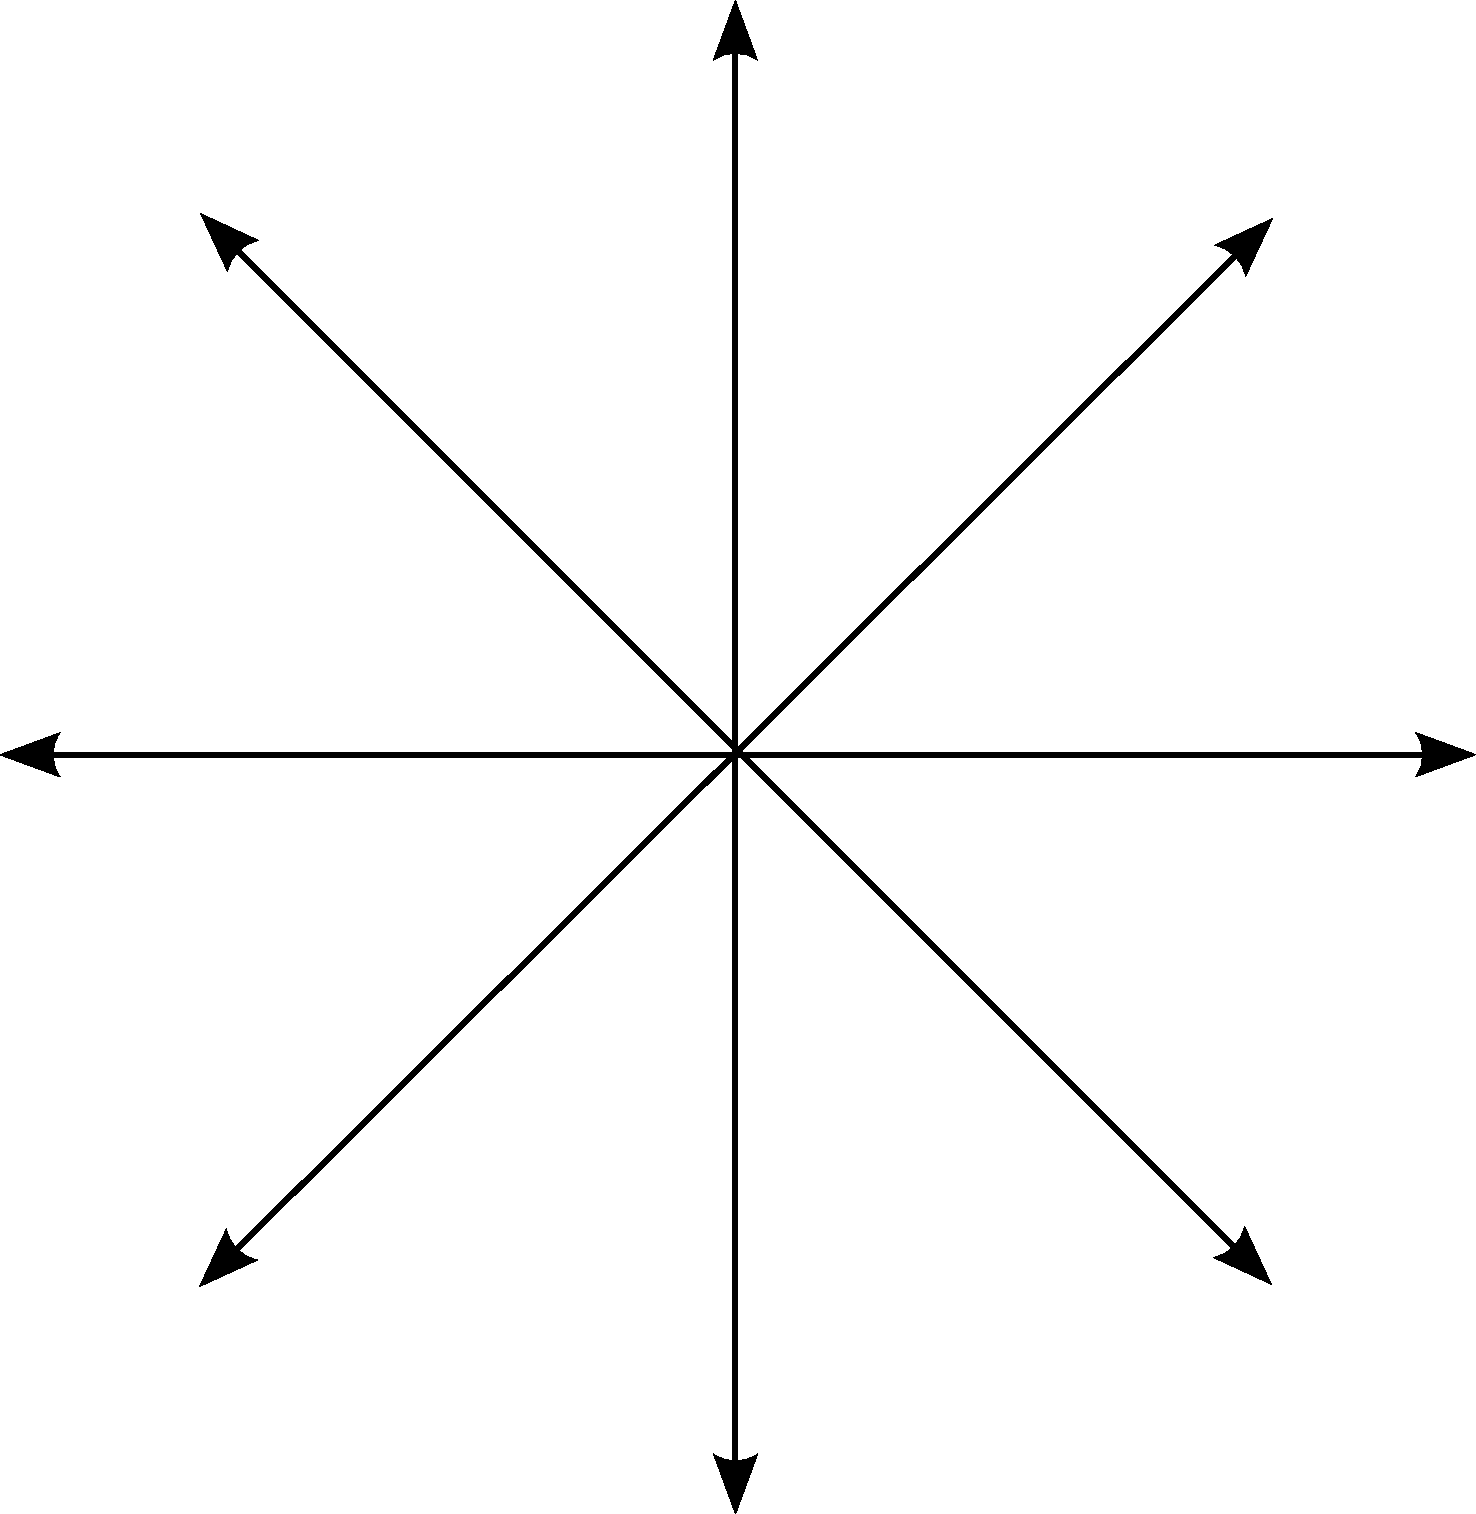
\includegraphics[scale=0.15]{Imatges/figuraE21-5} 
\end{center}
\noindent
\rule{\textwidth}{3pt}
\index{A!utilitzar moviments absoluts amb|)}
\index{lletra A!utilitzar moviments absoluts amb|)}
\index{moviments absoluts!significat de|)}
\index{punts!moviments ab@i moviments absoluts|)}
\index{punts!utilitzar negated amb els mètodes setX:setY:}

\section{Bucles i translacions}
\index{oques volant, patrons de|(}
\index{translacions!bucles@i bucles|(}
\index{bucles!translacions@i translacions|(}
Abans de continuar llegint, intenteu definir un \emph{script} que dibuixi la figura~\ref{fig2104}.
\begin{figure}[h!]
\begin{center}
\includegraphics[scale=0.4]{Imatges/figura21-4.png}
\end{center}
\caption{Un patró d'oques volant.}
\label{fig2104}
\end{figure}

La nostra solució apareix a l'\emph{Script}~\ref{scr21-16}, que dibuixa la figura~\ref{fig2104}. Els punts defineixen un cert nombre de mètodes útils, com per exemple \textsf{negated} i \textsf{setX:setY:}:\index{negated mètode, utilitzar en punts}
\begin{itemize}
\item El mètode \textsf{negated} enviat a un punt retorna un altre punt les coordenades \emph{x} i \emph{y} del qual són els valors negats  del punt receptor. Així, el punt \textsf{(200@400) negated} és el punt \textsf{-200@-400}. Fixeu-vos que els parèntesis són necessaris. De fet, \textsf{negated} és també un mètode entès pels nombres. Així, l'expressió \textsf{200@400 negated} dóna com a resultat el punt \textsf{200@-400} (un punt fora de la pantalla)., ja que el mètode \textsf{negated}, sent un mètode unari, és executat pel nombre \textsf{400} abans d'executar-se el mètode \textsf{@}. A l'\emph{Script}~\ref{scr21-16}, aquest mètode és utilitzat per produir una translació en la direcció oposada.
\item El mètode \textsf{setX:setY:} canvia les coordenades d'un punt. Així, després d'executar l'expressió \textsf{unPunt setX: 200 setY: 400}, el punt \textsf{unPunt} té coordenada \emph{x} \textsf{200} i coordenada \emph{y} \textsf{400}. \index{setX:setY: mètode, utilitzar en punts}
\end{itemize}

\begin{script}  Un patró fet d'oques volant
\textsf{\upshape
\begin{tabbing}
\hspace{10mm} \= \hspace{5mm} \= \hspace{5mm} \= \kill
$|$ pica punt1 mou desplacament $|$\\
punt1 := 200@300.\\
mou := 25@0.\\
desplacament := -25@50.\\
pica := Bot nou.\\
5 vegadesRepetir:\\
\> [ 10 vegadesRepetir: \\
\>\> [ pica \\
\>\>\> triangleA: punt1 \\
\>\>\> delta1: -25@-25\\
\>\>\> delta2: -25@25.\\
\>\> punt1 := punt1 + mou ].\\
\> punt1 := punt1 + desplacament.\\
\> mou := mou negated.\\
\> desplacament setX: desplacament x negated setY: desplacament y ]. \\
\end{tabbing}}
\label{scr21-16}
\end{script}

L'\emph{Script}~\ref{scr21-16} utilitza els mètodes \textsf{negated} i \textsf{setX:setY:} dins d'un doble bucle per generar el patró d'oques volant sobre una determinada regió de la pantalla. El bucle interior és fet de manera similar a l'\emph{Script}~\ref{scr21-12}, excepte que l'orientació del triangle i la de la translació han estat girades, de manera que la línia de triangles és ara horitzontal. El bucle exterior fa una translació del darrer triangle per posar-lo sobre de la línia de triangles tot just dibuixada, utilitzant la variable \textsf{desplacament}; després, la translació és invertida de manera que la línia següent és dibuixada en l'ordre capgirat. Els triangles, però, encara es dibuixen amb la mateixa orientació. El fet que una segona línia de triangles sembli apuntar en la direcció oposada és una il·lusió òptica provocada pel contacte que hi ha entre línies de triangles. Fixeu-vos que la variable \textsf{desplacament} ha de ser transformada d'una manera especial: el signe de la seva coordenada \emph{x} és invertit al final de cada línia per compensar la darrera translació, que no es dibuixa.\index{oques volant, patrons de|)} \index{bucles!translacions@i translacions|)} \index{translacions!bucles@i bucles|)}

\section{Més experiments}

\begin{center}
\colorbox{black}{\makebox[\textwidth]{  \color{white} {\large {\bfseries Experiment 21-6 (traslladar un robot a un punt)}}}}
\end{center}
\index{traslladar un robot a un punt, Experiment}
\index{Experiments!traslladar un robot a un punt}
\index{punts!traslladar robots a}
{\small
\noindent
Definir mètodes amb un comportament senzill i ben definit és una manera de simplificar el vostre codi, tal com vam explicar al capítol~\ref{cap16}. Com definiríeu un mètode \textsf{trasllada: unPunt} que trasllada el receptor, un robot, fins a \textsf{unPunt} des de la seva posició actual? Abans de consultar la nostra solució al Mètode~\ref{met21-1}, proveu de fer-ho vosaltres mateixos.}\\
\noindent
\rule{\textwidth}{3pt}

\begin{metode} Traslladar un Robot a un Punt
\noindent
\textsf{\upshape
\begin{tabbing}
\hspace{5mm} \= \hspace{10mm} \= \kill
{\bfseries trasllada: unPunt}\\
\> ``trasllada el receptor a unPunt''\\
\\
\> self vesA: (self center + unPunt)
\end{tabbing}
}
\label{met21-1}
\end{metode}

Proposeu un mètode diferent, \textsf{traslladaX: x y: y} que pren els valor d'\textsf{x} i d'\textsf{y} separadament com a arguments. \index{robots!traslladar a un punt}

\begin{center}
\colorbox{black}{\makebox[\textwidth]{  \color{white} {\large {\bfseries Experiment 21-7 (utilitzar el mètode trasllada: 1)}}}}
\end{center}
\index{utilitzar el mètode trasllada: 1, Experiment}
\index{Experiments!utilitzar el mètode trasllada: 1}
{\small
\noindent
Canvieu la definició del mètode \textsf{triangleA:punt2:punt3:} per tal que utilitzi el mètode \textsf{trasllada:unPunt}.}\\
\noindent
\rule{\textwidth}{3pt}

\begin{center}
\colorbox{black}{\makebox[\textwidth]{  \color{white} {\large {\bfseries Experiment 21-8 (utilitzar el mètode trasllada: 2)}}}}
\end{center}
\index{utilitzar el mètode trasllada: 2, Experiment}
\index{Experiments!utilitzar el mètode trasllada: 2}
{\small
\noindent
Utilitzant el mètode \textsf{trasllada:unPunt}, torneu a implementar alguns dels mètodes que heu fet en aquest capítol, i compareu-ne la mida i la complexitat.}\\
\noindent
\rule{\textwidth}{3pt}

\section{Resum}
\index{vesA: mètode!descripció i exemple}
\begin{itemize}
\item Un punt és un parell de nombres: tenen una coordenada \emph{x}, o coordenada horitzontal, i una coordenada \emph{y}, o coordenada vertical.
\item \textsf{200@400} és un punt la coordenada \emph{x} del qual és 200 i la coordenada \emph{y} del qual és 400.
\item El sistema de coordenades d'Smalltalk té el seu origen (0,0) a la cantonada superior esquerra de la pantalla, i l'eix \emph{y} té la seva direcció positiva cap avall.
\item Per evitar problemes amb els punts, envolteu-los de parèntesis quan participen en operacions complexes.
\item Els mètode \textsf{vesA: unPunt} i \textsf{saltaA: unPunt} fan que el receptor es mogui a la posició de l'argument, un punt.
\end{itemize}

\newpage

\noindent
Aquí teniu alguns dels mètodes associats als punts: \index{center (missatge), descripció i exemple} \index{saltaA: missatge, descripció i exemple} \index{punt1 $*$ nombre missatge, descripció i exemple} \index{punt1 + punt2 missatge, descripció i exemple}
\index{punt1 negated missatge, descripció i exemple} \index{x"@y missatge, descripció i exemple}

\vspace*{3mm}

\noindent
\setlength{\extrarowheight}{1mm}
{\small \begin{tabular}{p{30mm}p{60mm}p{40mm}}
\hline
\textbf{Missatge} & \textbf{Descripció} & \textbf{Exemple} \\
\hline
\textsf{{\itshape x @ y}} & Crea un punt a les coordenades donades. & \textsf{300 @ 600}\\
\textsf{vesA: unPunt} & Ordena al robot moure's a un punt donat. & \textsf{pica vesA: 300 @ 600}\\
\textsf{saltaA: unPunt} & Posiciona un robot en el punt donat. & \textsf{pica saltaA: 300 @ 600}\\
\textsf{punt1 + punt2} & Crea un punt les coordenades del qual són la suma de les coordenades dels dos punts donats. Això és útil per representar translacions.
& \textsf{(50@200) + (300@600)}\\
\textsf{punt1 $*$ nombre} & Crea un punt les coordenades del qual són els productes de les coordenades del punt i el nombre. & \textsf{(50@200)$*$3}\\
\textsf{punt1 negated} & Construeix un punt les coordenades del qual són les oposades de les coordenades del punt original. & \textsf{(50@200) negated}\\
\textsf{center} & Retorna la posició actual del robot com a punt. & \textsf{punt := pica center}\\
\hline
\end{tabular}}

\chapter{Comportament avançat dels robots}
\label{cap22}

Fins ara us havíem presentat només un subconjunt dels missatges que es poden enviar a un robot. En aquest capítol presentarem alguns missatges més avançats que utilitzarem en propers experiments.

\section{Obtenir la direcció d'un robot}
\index{direcció!obtenir pels robots}
\index{robots!obtenir direcció pels robots}
El primer mètode que ens cal és el mètode \textsf{direccio}, que retorna la direccio actual del robot en graus. Utilitzant aquest missatge podeu verificar que els missatges \textsf{nord}, \textsf{sud}, etc. que modifiquen la direcció del robot d'una manera absoluta estan d'acord amb les seves definicions matemàtiques, com veieu a l'\emph{Script}~\ref{scr22-1} i s'il·lustra a la figura~\ref{fig2201}. Fixeu-vos que la direcció és sempre un nombre entre -179 i 180 graus.

\begin{script}  Il·lustrar el mètode \textsf{\upshape direccio}
\textsf{\upshape
\begin{tabbing}
\hspace{10mm} \= \hspace{5mm} \= \hspace{5mm} \= \kill
$|$ robot $|$\\
robot := Bot nou.\\
robot nord.\\
robot direccio.\\
{\itshape -- Escriure el valor retornat: 90}\\
robot oest.\\
robot direccio.\\
{\itshape -- Escriure el valor retornat: 180}\\
robot est.\\
robot direccio.\\
{\itshape -- Escriure el valor retornat: 0}\\
robot sudEst.\\
robot direccio.\\
{\itshape -- Escriure el valor retornat: -45}
\end{tabbing}}
\label{scr22-1}
\end{script}

\section{Apuntar en una direcció}
\index{direcció!apuntar en una|(}
\index{giraA: mètode; efecte de|(}
El missatge \textsf{giraA: {\itshape unaDireccio}} li diu al receptor que giri cap a una determinada direcció donada com un angle en graus. Hem anomenat l'argument d'aquest missatge \textsf{{\itshape unaDireccio}} més que \textsf{{\itshape unAngle}} per emfatitzar el fet que el paràmetre representa un angle absolut, basat en la definició matemàtica il·lustrada a la figura~\ref{fig2201}. Així, per exemple, el missatge \textsf{giraA: 45} gira el robot receptor al nordest, sense importar on apuntava abans. Compareu amb el missatge \textsf{gira: 45}, que gira el robot 45 graus a l'esquerra \emph{relatius a la posició actual}. Això significa que l'expressió \textsf{robot giraA: 90} és equivalent a totes les següents expressions: \textsf{robot nord}, \textsf{robot giraA: -270} i \textsf{robot giraA: 90 + 360} (veieu l'\emph{Script}~\ref{scr22-2}). Fixeu-vos que els nombres a la figura~\ref{fig2201} són els més petits en valor absolut per representar un angle, i de fet, la implementació d'Smalltalk sempre fa que el robot giri aquesta quantitat mínima. \index{angles!per missatges referents a direccions absolutes} \index{giraA: unAngleAbsolutEnGraus, missatge; codi del}
\begin{figure}[h!]
\begin{center}
\includegraphics[scale=0.2]{Imatges/figura22-1}
\end{center}
\caption{Els angles associats amb els missatges de direccions absolutes.}
\label{fig2201}
\end{figure}
\newpage
\begin{script}  Il·lustrar el mètode \textsf{\upshape giraA: unAngleAbsolutEnGraus}
\textsf{\upshape
\begin{tabbing}
\hspace{10mm} \= \hspace{5mm} \= \hspace{5mm} \= \kill
$|$ robot $|$\\
robot := Bot nou.\\
robot giraA: 90.\\
{\itshape ``dóna el mateix resultat que: robot nord''}\\
\end{tabbing}}
\label{scr22-2}
\end{script}
\index{direccions absolutes!angles associats amb}
\section{Distància des d'un punt}
\index{giraA: mètode; efecte de|)}
\index{direcció!apuntar en una|)}
\index{punts!distància des d'un}
La propera informació que voldríem obtenir d'un robot és la seva distància a un punt donat. Això és precisament el que obteniu quan envieu el missatge \textsf{distanciaDesde: {\itshape unPunt}} a un robot. Aquesta informació és útil, per exemple, quan volem saber si un robot s'està apropant a un lloc determinat. \index{distanciaDesde: missatge!codi per}

\begin{script}  Il·lustrar \textsf{\upshape distanciaDesde: unPunt}
\textsf{\upshape
\begin{tabbing}
\hspace{10mm} \= \hspace{5mm} \= \hspace{5mm} \= \kill
$|$ robot $|$\\
robot := Bot nou.\\
robot saltaA: 100@100.\\
robot distanciaDesde: (140@130).\\
{\itshape -- Escriure el valor retornat: 50}\\
\end{tabbing}}
\label{scr22-3}
\end{script}

\section{Tornar al centre de la pantalla}
\index{robots!tornar al centre de la pantalla}
\index{pantalla!posicionar robots al centre de la}
Un altre missatge útil és \textsf{origen}, que posiciona el robot receptor al lloc on va aparèixer quan es va crear, és a dir, al centre de la pantalla. \index{origen, missatge; efecte de}

\section{Posició si es mogués}

Algunes vegades ens agradaria conèixer la posició que un robot ocuparia si es mogués una determinada distància en la seva direcció actual. Utilitzarem molt aquesta funcionalitat quan simulem comportament animal. Per a això s'ha definit el mètode \textsf{posicioSiVes: unaDistancia} i es pot utilitzar com veieu a l'\emph{Script}~\ref{scr22-4}.\index{posició!especular amb}
\newpage
\begin{script}  Il·lustrar \textsf{\upshape posicioSiVes: unaDistancia}
\textsf{\upshape
\begin{tabbing}
\hspace{10mm} \= \hspace{5mm} \= \hspace{5mm} \= \kill
$|$ robot $|$\\
robot := Bot nou.\\
robot saltaA: 100@100.\\
robot est.\\
robot posicioSiVes: 100.\\
{\itshape -- Escriure el valor retornat: 200@100}\\
\end{tabbing}}
\index{posicioSiVes: mètode, codi per}
\label{scr22-4}
\end{script}

\subsection{En una capsa}
\index{capses!moure robots dins de|(}
\index{rectangles!moure robots dins de|(}
\index{robots!moure dins de|(}
Abans de llegir-ne la solució, proveu de definir un mètode \textsf{ves: unEnter siDinsCapsa: unRectangle} que mou el receptor només si aquest moviment no el posiciona fora d'un determinat rectangle, com veieu a l'\emph{Script}~\ref{scr22-5}.\index{ves:siDinsCapsa: mètode, codi per al}

\begin{script}  Il·lustrar \textsf{\upshape ves: unEnter siDinsCapsa: unRectangle}
\textsf{\upshape
\begin{tabbing}
\hspace{10mm} \= \hspace{5mm} \= \hspace{5mm} \= \kill
Bot nou\\
\> ves: 100\\
\> siDinsCapsa: (Rectangle center: World center extent: 400@300)
\end{tabbing}}
\label{scr22-5}
\end{script}

Per crear el rectangle podeu utilitzar, per exemple, el mètode \textsf{center:extent:}, que crea un rectangle centrat en un punt. L'expressió \textsf{(Rectangle center: World center extent: 400@300)} retorna un rectangle  el centre del qual és el centre de la pantalla i la base i l'altura del qual són 400 i 300 píxels. Podeu demanar a un rectangle si conté un punt utilitzant el mètode \textsf{containsPoint: unPunt}. Per determinar quina seria la posició del robot si es mogués endavant una distància determinada podeu utilitzar el mètode \textsf{posicioSiVes: unaDistancia}. \index{rectangles!dibuixar}

El Mètode~\ref{met22-1} us mostra la definicio de \textsf{ves: unEnter siDinsCapsa: unRectangle}. Utilitza el mètode \textsf{posicioSiVes:}, que calcula la posició del robot si s'hagués de moure endavant una determinada distància en la seva direcció actual. Farem servir la idea de restringir el moviment del robot per representar comportament animal al capítol~\ref{cap23}.\index{receptors!moure si va a parar dins d'un rectangle}

\begin{metode} Mou el receptor només si anirà a parar dins d'un rectangle donat
\noindent
\textsf{\upshape
\begin{tabbing}
\hspace{5mm} \= \hspace{10mm} \= \kill
ves: unEnter siDinsCapsa: unRectangle\\
\> ``mou endavant el receptor només si roman dins un rectangle''\\
\\
\> (unRectangle containsPoint: (self posiciosSiVes: unEnter))\\
\>\> siCert: [ self ves: unEnter. ]
\end{tabbing}
}
\label{met22-1}
\end{metode}

\section{Apuntar cap a un punt}
\index{robots!moure dins de|)}
\index{capses!moure robots dins de|)}
\index{rectangles!moure robots dins de|)}
\index{direccio mètode!exemple de|(}
\index{direcció!apuntar cap a una|(}
\index{punts!apuntar cap a un|(}
De vegades és necessari demanar a un robot que es dirigeixi cap a un punt determinat. El mètode \textsf{apuntaA: unPunt} canvia la direcció del receptor de manera que apunti en la direcció del punt \textsf{unPunt}. Un cop el mètode s'ha executat, el robot receptor apunta en la direcció del punt especificat, com veieu a la figura~\ref{fig2202}. Podeu verificar-ho utilitzant el mètode \textsf{direccio}, tal com mostrem als \emph{Scripts}~\ref{scr22-6} i ~\ref{scr22-7}.
\begin{figure}[h!]
\begin{center}
\includegraphics[scale=0.5]{Imatges/figura22-2}
\end{center}
\caption{Un robot apunta al punt \textsf{\upshape 200@100} després d'haver-li enviat el missatge \textsf{\upshape apuntaA:}.}
\label{fig2202}
\end{figure}

\begin{script}  Il·lustrar \textsf{\upshape apuntaA: unPunt}
\textsf{\upshape
\begin{tabbing}
\hspace{10mm} \= \hspace{5mm} \= \hspace{5mm} \= \kill
$|$ robot $|$\\
robot := Bot nou.\\
robot saltaA: 100@200.\\
robot apuntaA: 200@100.\\
robot direccio\\
{\itshape -- Escriure el valor retornat: 45}
\end{tabbing}}
\index{apuntaA: mètode!codi de|(}
\label{scr22-6}
\end{script}

\begin{script}  Il·lustrar \textsf{\upshape apuntaA: unPunt}
\textsf{\upshape
\begin{tabbing}
\hspace{10mm} \= \hspace{5mm} \= \hspace{5mm} \= \kill
$|$ robot $|$\\
robot := Bot nou.\\
robot saltaA: 100@200.\\
robot apuntaA: 200@300.\\
robot direccio\\
{\itshape -- Escriure el valor retornat: -45}
\end{tabbing}}
\label{scr22-7}
\end{script}

Tot i així, ser capaç d'apuntar a un lloc donat pot no ser suficient. De vegades, ens agradaria conèixer l'angle que hauria de girar un robot per apuntar a una posició determinada. El mètode \textsf{anglePerApuntarA: unPunt} retorna la diferència entre la direcció actual del receptor i la direcció amb què apuntaria cap a \textsf{unPunt}.\index{anglePerApuntarA: mètode!diagrama de i codi de}\index{apuntaA: mètode!codi de|)}

La figura~\ref{fig2203} i l'\emph{Script}~\ref{scr22-8} il·lustren aquest mètode. A la figura, un robot està apuntant en la direcció del punt A, i la seva direcció és 45. Ara, l'expressió \textsf{anglePerApuntarA: 200@100} retorna \textsf{0}, perque el robot \emph{ja} està apuntant cap a aquest punt. Després el robot és girat cap al punt B. Ara l'expressió \textsf{anglePerApuntarA: 200@100} retorna -45, ja que el robot s'hauria de girar 45 graus en la direcció de les agulles del rellotge per apuntar cap al punt A.\index{direcció!apuntar cap a una|)}
\begin{figure}[h!]
\begin{center}
\includegraphics[scale=0.5]{Imatges/figura22-3}
\end{center}
\caption{El mètode \textsf{\upshape anglePerApuntarA: unPunt} retorna l'angle que el robot hauria de girar per apuntar a \textsf{\upshape unPunt}.}
\label{fig2203}
\end{figure}

\begin{script}  Il·lustrar \textsf{\upshape anglePerApuntarA:}. Veieu la figura~\ref{fig2203}.
\textsf{\upshape
\begin{tabbing}
\hspace{10mm} \= \hspace{5mm} \= \hspace{5mm} \= \kill
$|$ robot $|$\\
robot := Bot nou.\\
robot saltaA: 100@200.\\
robot apuntaA: 200@100.\\
robot direccio\\
{\itshape -- Escriure el valor retornat: 45}\\
robot anglePerApuntarA: 200@100.\\
{\itshape -- Escriure el valor retornat: 0}\\
robot apuntaA: 100@100.\\
robot anglePerApuntarA: 200@100.\\
{\itshape -- Escriure el valor retornat: -45}
\end{tabbing}}
\label{scr22-8}
\index{punts!apuntar cap a un|)}
\end{script}

\section{Centre versus posició}
\index{center (missatge), descripció i exemples}
\index{centre versus posició}
\index{direccio mètode!exemple de|)}
\index{posició!determinar la}
Finalment, pot ser que vulgueu conèixer la posició actual del robot a la pantalla. Per obtenir aquesta informació podeu fer servir el mètode \textsf{center}, que retorna la posició del llapis del robot. Un robot també entén el mètode \textsf{position}, proporcionat per Squeak, que retorna la cantonada superior esquerra del rectangle representant el robot, com mostrem a la figura~\ref{fig2204}. Usualment, no heu d'utilitzar el mètode \textsf{position}, que ve donat per Squeak i no és específic de la classe \textsf{Bot}. \index{posició actual dels robots, determinar} \index{robots!determinar la posició actual}
\begin{figure}[h!]
\begin{center}
\includegraphics[scale=0.35]{Imatges/figura22-4}
\end{center}
\caption{La diferència entre la posició i el centre d'un robot.}
\label{fig2204}
\end{figure}

\section{Resum}

La taula següent resumeix els mètodes introduïts en aquest capítol:\index{anglePerApuntarA: mètode!descripció i exemples de} \index{tornarInvisible i tornarVisible mètodes, efectes de} \index{direccio mètode!descripció i exemples de}
\index{distanciaDesde: missatge!descripció i exemple de} \index{posició!versus centre} \index{posició missatge, descripció i exemple de} \index{giraA: mètode; efecte de}

\vspace*{3mm}

\noindent
\setlength{\extrarowheight}{1mm}
{\small \begin{tabular}{p{37mm}p{50mm}p{50mm}}
\hline
\textbf{Missatge} & \textbf{Descripció} & \textbf{Exemple} \\
\hline
\textsf{anglePerApuntarA: unPunt} & 
Ordena al receptor calcular l'angle que hauria de girar per apuntar a \textsf{unPunt} & 
\textsf{berthe anglePerApuntarA: 100@100}\\
\textsf{giraA: unaDireccio} & 
Ordena al receptor girar en la direcció  \textsf{unaDireccio} & 
\textsf{berthe giraA: 90}\\
\textsf{direccio} & 
Ordena al receptor informar de la seva direcció actual & 
\textsf{berthe nord; direccio}\\
\textsf{position} & 
Ordena al receptor comunicar quina és la seva cantonada superior esquerra & 
\textsf{berthe position}\\
\textsf{center} & 
Ordena al receptor informar de la posició del seu llapis & 
\textsf{berthe center}\\
%\textsf{tornarVisible} & 
%Ordena al receptor mostrar-se & 
%\textsf{berthe tornarVisible}\\
%\textsf{tornarInvisible} & 
%Ordena al receptor amagar-se & 
%\textsf{berthe tornarInvisible}\\
\textsf{distanciaDesde: unPunt} & 
Ordena al receptor informar de la seva distància a \textsf{unPunt} &  
\textsf{berthe distanciaDesde: 140@130}\\
\hline
\end{tabular}}

\chapter{Simular comportament animal}
\label{cap23}

\includegraphics[scale=0.625]{Imatges/figura23-0}

Els ordinadors són bons per modelitzar el món en què vivim, des del creixement de les plantes fins a models del comportament dels mercats en ciències econòmiques. En aquest capítol us ensenyarem com modelitzar determinats comportaments animals i a utilitzar la simulació per entendre els factors que influencien aquests comportaments. Modelitzarem algunes estratègies que els animals utilitzen per caminar, escapar-se, trobar menjar i romandre en un entorn favorable. 

\section{Vagar}
\index{simulacions de comportament animal!vagar|(}
\index{vagar, simular|(}
Comencem modelitzant com podria vagar un animal. L'aproximació bàsica per simular el comportament vagant d'un animal és escriure un bucle en el qual l'animal camina i gira una mica a l'atzar. Utilitzarem un nombre aleatori en definir el mètode \textsf{vagant: unNombre}, que fa que el receptor camini un nombre aleatori de passos, giri un angle aleatori i repeteixi aquests moviments \textsf{unNombre} vegades (per obtenir un nombre aleatori entre 1 i 30, cal enviar el missatge \textsf{atRandom} al nombre \textsf{30}). Un resultat possible d'executar el mètode el podeu veure a la figura~\ref{fig2301}.
\begin{figure}[h!]
\begin{center}
\includegraphics[scale=0.5]{Imatges/figura23-1}
\end{center}
\caption{Un animal vaga caminant un nombre aleatori de passos i després girant a l'atzar.}
\label{fig2301}
\end{figure}

El Mètode~\ref{met23-1} presenta una manera de definir el comportament senzill descrit més amunt i il·lustrat a la figura. Aquí simplement ordenem al robot que es mogui aleatòriament una distància entre 1 i 30 píxels i que giri un angle entre 1 i 30 graus. L'\emph{Script}~\ref{scr23-1} mostra com fer servir aquest mètode.

\begin{script}  
\textsf{\upshape
\begin{tabbing}
\hspace{10mm} \= \hspace{5mm} \= \hspace{5mm} \= \kill
Bot nou vagant: 500
\end{tabbing}}
\label{scr23-1}
\end{script}

\begin{metode}
\noindent
\textsf{\upshape
\begin{tabbing}
\hspace{5mm} \= \hspace{10mm} \= \kill
{\bfseries vagant: n}\\
\> ``Fer moure el robot una distància aleatòria i girar un angle a l'atzar n vegades''\\
\> n vegadesRepetir:\\
\>\> [ self ves: 30 atRandom.\\
\>\> self giraEsquerra: 30 atRandom ]
\end{tabbing}}
\label{met23-1}
\end{metode}

Naturalment, els animals no vaguen a l'atzar. Eons de desenvolupament evolutiu han creat animals que es mouen i giren en resposta a estímuls del seu entorn. Potser un animal gira i vaga fins que succeeix un cert esdeveniment . Per començar a modelitzar aquest comportament, que l'animal repeteix fins que passa un esdeveniment determinat, modelitzat aquí com un clic d'un botó del ratolí per part de l'usuari, podríeu utilitzar un bucle condicional. El mètode \textsf{vagantFinsBotoPitjat} (Mètode~\ref{met23-2}) il·lustra aquest aspecte del model. Permet vagar a un animal fins que l'usuari pitgi un dels botons del ratolí. Com que el bucle és executat molt ràpidament, pot passar que l'ordinador sembli bloquejat, per tant continueu pitjant el botó fins que s'aturi.

\begin{metode} Un animal vaga a l'atzar fins que succeeix un esdeveniment.
\noindent
\textsf{\upshape
\begin{tabbing}
\hspace{5mm} \= \hspace{10mm} \= \kill
{\bfseries vagantFinsBotoPitjat}\\
\> ``Fer moure el robot una distància aleatòria i girar un angle a l'atzar \\
\> fins que un botó del ratolí sigui pitjat''\\
\\
\> [ self anyButtonPressed ] mentreFals:\\
\>\> [ self ves: 30 atRandom.\\
\>\> self giraEsquerra: 30 atRandom ]
\end{tabbing}}
\label{met23-2}
\end{metode}

\subsection{Separar influències}
\index{angles!aleatoris, per simular comportament animal|(}
El Mètode~\ref{met23-1} és interessant, però barreja dos aspectes del vagar de l'animal: el moviment a l'atzar i els canvis de direcció aleatoris. És més, cada cop que voleu provar un valor nou per a l'angle o el nombre de passos, heu de recompilar el mètode \textsf{vagant: n}. Així, definiu un mètode \textsf{vagant: n maxAngle: unAngle} que pren com a segon argument el valor màxim de l'angle aleatori que el receptor hauria de girar. En aquest mètode, feu que el robot sempre es mogui endavant una distància constant. Aquest mètode es pot utilitzar com veieu a l'\emph{Script}~\ref{scr23-2}.

\begin{script}  
\textsf{\upshape
\begin{tabbing}
\hspace{10mm} \= \hspace{5mm} \= \hspace{5mm} \= \kill
Bot nou vagant: 500 maxAngle: 60
\end{tabbing}}
\label{scr23-2}
\end{script}

Proveu d'endevinar quin aspecte tindrà la traça deixada per l'animal abans d'executar els vostres \emph{scripts}. Experimenteu amb diferents valors pels angles. Les figures~\ref{fig2302} i ~\ref{fig2303} mostren resultats diferents amb 15, 60, 90, 180 i 360 graus. \index{traces!endevinar les generades pel moviment dels animals}

\begin{figure}[h!]
\begin{center}
\includegraphics[scale=0.4]{Imatges/figura23-2}
\end{center}
\caption{Caminant amb angles aleatoris de com a molt 15 (esquerra), 60 (mig) i 90 (dreta) graus.}
\label{fig2302}
\end{figure}

\begin{figure}[h!]
\begin{center}
\includegraphics[scale=0.4]{Imatges/figura23-3}
\end{center}
\caption{Caminant amb angles aleatoris de com a molt 180 (esquerra) i 360 (dreta) graus.}
\label{fig2303}
\end{figure}

\subsection{Estudiar la influència de la longitud}
\index{angles!aleatoris, per simular comportament animal|)}
\index{longitud, examinar la influència en el moviment de vagar de la}
Hem estat jugant amb la influència de l'angle en la forma del recorregut. Quines hipòtesis teniu sobre la influència de la longitud? Què hauria de passar si un animal caminés una distància aleatòria i després girés un angle constant?

\subsection{Estudiar la influència del costat cap a on gira l'animal}
\index{girs, examinar en el comportament animal|(}
Fins ara, el nostre animal sempre ha girat cap a l'esquerra. Podem estudiar la influència de l'habilitat de girar només cap a un costat o cap als dos costats. Proveu de pensar una solució a aquest problema de programació abans de llegir-ne la nostra. Ajuda: Fixeu-vos que \textsf{atRandom} retorna un nombre entre el receptor i 1. Per tant, \textsf{2 atRandom} retorna o bé 1 o bé 2.

Una possible manera de generar una elecció aleatòria és introduint un nombre aleatori (1 o 2) per representar el costat cap a on es girarà, com s'esbossa a l'\emph{Script}~\ref{scr23-3}. Una altra idea és generar un nombre aleatori com a màxim el doble de l'angle màxim desitjat i restar-ne aquest angle. Per exemple, per obtenir un nombre entre -45 i 45, podeu generar un nombre aleatori entre 1 i 91 i restar-ne 46, com veieu a l'\emph{Script}~\ref{scr23-4}. La figura~\ref{fig2304} mostra què podria passar si utilitzéssim aquestes estratègies, i podeu veure que el recorregut sembla molt més el d'un animal real, diguem un cargol, que els recorreguts anteriors.
\begin{figure}[h!]
\begin{center}
\includegraphics[scale=0.5]{Imatges/figura23-4}
\end{center}
\caption{Un animal vaga caminant i girant a l'atzar, on és igualment probable girar a l'esquerra i girar a la dreta.}
\label{fig2304}
\end{figure}

\begin{script}  Un nombre aleatori (1 o 2) determina si l'animal gira a la dreta o a l'esquerra.
\textsf{\upshape
\begin{tabbing}
\hspace{10mm} \= \hspace{5mm} \= \hspace{5mm} \= \kill
\dots \\
\> esquerra := 2 atRandom.\\
\> esquerra = 1\\
\>\> siCert: [ self giraEsquerra: \dots ]\\
\>\> siFals: [ self giraDreta: \dots ]\\
\dots
\end{tabbing}}
\label{scr23-3}
\end{script}
\newpage
\begin{script}  L'angle màxim de gir es resta d'un nombre aleatori per donar com a resultat un angle que pot ser tant negatiu com positiu.
\textsf{\upshape
\begin{tabbing}
\hspace{10mm} \= \hspace{5mm} \= \hspace{5mm} \= \kill
\dots \\
\> rdAngle := ((1 + (angle $*$ 2)) atRandom) - (1 + angle).\\
\> self gira: rdAngle.\\
\dots
\end{tabbing}}
\label{scr23-4}
\end{script}

\section{Atrapat dins una capsa}
\index{vagar, simular|)}
\index{girs, examinar en el comportament animal|)}
\index{comportament d'un animal atrapat dins d'una capsa|seealso{capses}}
\index{comportament d'un animal atrapat dins d'una capsa!panorama general|(}
\index{rectangles|seealso{capses; rectangles d'or}}
\index{rectangles!centrats en animals}
\index{simulacions de comportament animal!vagar|)}
\index{simulacions de comportament animal!atrapat dins una capsa|(}
Ara ens agradaria restringir el moviment de l'animal de manera que romangui dins d'una capsa. Això ens permetrà estudiar estratègies diferents que aparentment alguns insectes fan servir quan es troben en una situació similar. Fer-ho és senzil. Abans d'ordenar l'animal que es mogui una certa distància, cal comprovar si la posició on anirà a parar és dins de la capsa. Aquest moviment restringit ja es va presentar al capítol~\ref{cap22}, amb el Mètode~\ref{met22-1}, però repetirem el codi en el Mètode~\ref{met23-3}

\begin{metode} 
\noindent
\textsf{\upshape
\begin{tabbing}
\hspace{5mm} \= \hspace{10mm} \= \kill
{\bfseries ves: unaDistancia siDinsCapsa: unRectangle}\\
\> ``mou endavant el receptor només si roman dins un rectangle''\\
\> (unRectangle containsPoint: (self posiciosSiVes: unaDistancia))\\
\>\> siCert: [ self ves: unaDistancia. ]
\end{tabbing}}
\label{met23-3}
\end{metode}

Per crear una capsa, podem crear un rectangle, com veieu a l'\emph{Script}~\ref{scr23-5}. Aquest \emph{script} crea una capsa de costat 200 píxels al voltant de la posició actual de l'animal.

\begin{script}  Crear un rectangle centrat en un animal.
\textsf{\upshape
\begin{tabbing}
\hspace{10mm} \= \hspace{5mm} \= \hspace{5mm} \= \kill
$|$ pica rectangle $|$\\
pica := Bot nou.\\
rectangle := Rectangle center: pica center extent: 200@200.\\
\end{tabbing}}
\label{scr23-5}
\end{script}

Per millorar visualment la simulació, i si voleu veure la capsa a la pantalla, heu de crear un ``rectangle morph'', és a dir, un objecte gràfic la forma del qual és un rectangle, com fem a l'\emph{Script}~\ref{scr23-6}. Aquest \emph{script} primer crea un rectangle, i després crea un \emph{rectangle morph} afitat pel rectangle, amb l'interior transparent i un costat blau. Finalment, dibuixem el \emph{rectangle morph} amb el mètode \textsf{openInWorld}.

\begin{script}  Visualitzar un rectangle centrat en un animal.
\textsf{\upshape
\begin{tabbing}
\hspace{10mm} \= \hspace{5mm} \= \hspace{5mm} \= \kill
$|$ pica rectangle rm $|$
pica := Bot nou.\\
rectangle := Rectangle center: pica center extent: 200@200.\\
rm := RectangleMorph new.\\
rm bounds: rectangle.\\
rm color: Color transparent.\\
rm setBorderWidth: 2 borderColor: Color blau.\\
rm openInWorld.
\end{tabbing}}
\label{scr23-6}
\end{script}

Ara definirem el mètode \textsf{capsa: unRectangle} que dibuixa una capsa representant el rectangle, ja que l'utilitzareu molt.

\begin{metode} 
\noindent
\textsf{\upshape
\begin{tabbing}
\hspace{5mm} \= \hspace{10mm} \= \kill
{\bfseries capsa: unRectangle}\\
\> ``Dibuixa un \emph{morph} per representar el rectangle''\\
\> $|$ rm $|$\\
\> rm := RectangleMorph new.\\
\> rm bounds: unRectangle.\\
\> rm color: Color transparent.\\
\> rm setBorderWidth: 2 borderColor: Color blau.\\
\> rm openInWorld.
\end{tabbing}}
\label{met23-4}
\end{metode}

Ara ja podem combinar totes les peces per crear un animal dins de la capsa i comprovar el mètode \textsf{ves: unaDistancia siDinsCapsa: unRectangle}. La propera qüestió és: Com podem modelitzar més fidelment el comportament d'un animal tancat? Imagineu diferents alternatives. Hauríeu d'experimentar amb unes quantes variacions.

\subsection{Resseguir els costats}
\index{girs, examinar en el comportament animal|(}
\index{comportament d'un animal atrapat dins d'una capsa!panorama general|)}
\index{comportament d'un animal atrapat dins d'una capsa!resseguir els costats|(}
\index{costats, examinar en el comportament d'un animal tancat en una capsa|(}
Una aproximació possible és fer que l'animal giri una miqueta quan no es pot moure, i ho torni a provar. Això és el que fem amb el Mètode~\ref{met23-5}. Quan el robot es pot moure, només vaga, però si el seu moviment el faria sortir de la capsa, gira un cert angle. Aquest moviment és dins d'un bucle que fa que el robot giri i torni a provar de moure's. Si el gir no és prou gran, continua girant fins que es pot moure altre cop.

Els \emph{Scripts}~\ref{scr23-6} i~\ref{scr23-7} junts produeixen resultats similars als resultats que podeu veure a la figura~\ref{fig2305}. L'\emph{Script}~\ref{scr23-6} mostra un \emph{morph} rectangular per fer aparèixer la capsa i l'\emph{Script}~\ref{scr23-7} controla el moviment de l'animal.
\begin{figure}[h!]
\begin{center}
\includegraphics[scale=0.5]{Imatges/figura23-5}
\end{center}
\caption{Un animal tancat dins d'una capsa gira fins que es pot moure sense xocar amb un costat.}
\label{fig2305}
\end{figure}

\begin{script} Un animal tancat en una capsa prova de moure's
\textsf{\upshape
\begin{tabbing}
\hspace{10mm} \= \hspace{5mm} \= \hspace{5mm} \= \kill
$|$ t rec $|$\\
t := Bot nou.\\
rec := (Rectangle center: t center extent: 200@200).\\
t ressegueix: 500 costatDeCapsa: rec
\end{tabbing}}
\label{scr23-7}
\end{script}

\begin{metode} El robot gira si no es pot moure i torna a provar-ho.
\noindent
\textsf{\upshape
\begin{tabbing}
\hspace{5mm} \= \hspace{5mm} \= \hspace{5mm} \= \kill
{\bfseries ressegueix: n costatDeCapsa: unRectangle}\\
\> self capsa: unRectangle.\\
\> n vegadesRepetir:\\
\>\> [ (unRectangle containsPoint: (self posicioSiVes: 30))\\
\>\>\> siCert: [ \= self ves: 30.\\
\>\>\>\> self giraEsquerra: 30 atRandom  ]\\
\>\>\> siFals: [ self giraEsquerra: 1  ]  ]
\end{tabbing}}
\label{met23-5}
\end{metode}

\subsection{Volar al costat oposat}
\index{costats, examinar en el comportament d'un animal tancat en una capsa|)}
\index{comportament d'un animal atrapat dins d'una capsa!volar al costat oposat}
\index{comportament d'un animal atrapat dins d'una capsa!resseguir els costats|)}
Una altra estratègia per simular és la de l'insecte que prova de volar fins al costat oposat. Us deixarem programar-ho a vosaltres mateixos,en teniu una possible traça a l'esquerra de la figura~\ref{fig2306}.
\begin{figure}[h!]
\begin{center}
\includegraphics[scale=0.5]{Imatges/figura23-6}
\end{center}
\caption{\emph{Esquerra:} L'insecte es mou en la direcció oposada quan es troba amb una paret.
\emph{Dreta:} L'insecte tria una direcció a l'atzar quan es troba amb una paret. Aquesta figura es va obtenir amb un valor màxim de moviment de 10 píxels i girant un màxim de 90 graus. Per escapar, farà un gir aleatori d'un màxim de 360 graus.}
\label{fig2306}
\end{figure}

\subsection{Direcció aleatòria}
\index{comportament d'un animal atrapat dins d'una capsa!direcció aleatòria}
\index{direcció!aleatòria pel comportament animal}
Una altra possibilitat per canviar la direcció de l'animal és fer-ho a l'atzar. Us deixarem definir aquest comportament, pel qual teniu una possible traça a la dreta de la figura~\ref{fig2306}. \index{girs, examinar en el comportament animal|)}

\subsection{Afegir una sortida a la capsa}
\index{capses|seealso{comportament d'un animal atrapat dins d'una capsa}}
\index{rectangles!com a sortides d'un animal atrapat dins d'una capsa}
\index{capses!afegint una sortida a}
\index{comportament d'un animal atrapat dins d'una capsa!afegir una sortida a la capsa}
Ara podeu afegir un altre rectangle per representar la sortida de la capsa, tal com està il·lustrat a l'\emph{Script}~\ref{scr23-8} i podeu veure a la figura~\ref{fig2307}.
\begin{figure}[h!]
\begin{center}
\includegraphics[scale=0.5]{Imatges/figura23-7}
\end{center}
\caption{Una capsa amb una sortida.}
\label{fig2307}
\end{figure}

\begin{script} Visualitzar una capsa amb una sortida.
\textsf{\upshape
\begin{tabbing}
\hspace{10mm} \= \hspace{5mm} \= \hspace{5mm} \= \kill
$|$ box rm rm2 exit $|$\\
box := Rectangle center: World center extent: 200@200.\\
rm := RectangleMorph new.\\
rm bounds: box.\\
rm color: Color transparent.\\
rm setBorderWidth: 2 borderColor: Color blau.\\
rm openInWorld.\\
exit := Rectangle origin: (box topRight + (0@50)) extent: 100@100.\\
rm2 := RectangleMorph new.\\
rm2 bounds: exit.\\
rm2 color: Color transparent.\\
rm2 setBorderWidth: 2 borderColor: Color negre.\\
rm2 openInWorld.
\end{tabbing}}
\label{scr23-8}
\end{script}

Definiu un mètode per estalviar-vos de repetir aquest codi més d'una vegada. Podríeu crear un mètode anomenat \textsf{escapant: unaCapsa ambSortida: unaSortida} que primer comprovaria si el proper moviment estaria contingut dins el rectangle que representa la sortida, i si aquest fos el cas, el mètode deixaria escapar l'animal.\index{simulacions de comportament animal!atrapat dins una capsa|)} \index{escapant:ambSortida: mètode, crear}

\section{Romandre en un entorn segur}
\index{bacteris, exemple!canviar direcció}
\index{bacteris, exemple!incrementar velocitat}
Us heu preguntat mai com és possible que els bacteris del llim romanguin sempre a prop de llocs humits, evitant els llocs secs? D'acord, potser no. Sigui com sigui, us proposem simular les estratègies que formes de vida bàsiques com els bacteris utilitzen per romandre en àrees on tenen més possibilitats de sobreviure. Us proposem que modelitzeu dues estratègies molt senzilles descobertes a finals dels anys 50 utilitzant només canvis en direcció i velocitat. Fixeu-vos que quan parlem de velocitat, volem dir la distància que l'animal es pot moure a cada pas, que en el nostre cas serà la distància en píxels que rep el mètode \textsf{ves:} com a argument.

La primera estratègia que els bacteris poden seguir és canviar de direcció a l'atzar en qualsevol circumstància però canviar de velocitat depenent del grau de seguretat de l'entorn. Aquesta estratègia té
sentit ja que, si un bacteri considera una regió segura, trigarà més temps a fer un determinat recorregut, i per tant romandrà més temps en un entorn segur que en un entorn insegur. Un possible recorregut per un bacteri es mostra a la figura~\ref{fig2308}.
\begin{figure}[h!]
\begin{center}
\includegraphics[scale=0.5]{Imatges/figura23-8}
\end{center}
\caption{Primera estratègia. El bacteri incrementa la seva velocitat quan es troba en un entorn insegur. Canvia de direcció amb una taxa constant. La velocitat en un entorn segur és un nombre aleatori com a molt gran de 25 píxels, mentre que en un entorn insegur és de 100 píxels. L'interior del rectangle representa l'entorn segur.}
\label{fig2308}
\end{figure}

La segona estratègia és l'oposada. El bacteri es mou a velocitat constant però canvia de velocitat en funció de la seguretat que li ofereix l'entorn. Canvia la seva direcció un angle en mitjana més gran en un entorn segur que en un entorn insegur. Per tant, té més possibilitats de tornar sobre els seus passos i romandre dins una regió més petita. Alguns bacteris molt senzills fan servir aquesta estratègia per romandre en entorns on poden trobar menjar. Un possible recorregut per a un bacteri d'aquestes característiques el podeu veure a la figura~\ref{fig2309}.
\begin{figure}[h!]
\begin{center}
\includegraphics[scale=0.5]{Imatges/figura23-9}
\end{center}
\caption{Segona estratègia. El bacteri incrementa el seu rang de canvi de direcció en un entorn segur. Aquí la velocitat és 25, i el canvi de direcció és com a màxim 36 en un entorn insegur i 360 en un de segur.}
\label{fig2309}
\end{figure}

Per implementar aquestes idees, només cal que us imagineu que el rectangle que hem estat utilitzant representa una regió segura. Per a la primera estratègia, podríeu definir un mètode anomenat \textsf{romanEnAngleConstantNVegades: unNombre dinsUn: unaRegio}, com veieu a l'\emph{Script}~\ref{scr23-9}. Experimenteu amb diferents valors de l'angle que pot girar el bacteri.\index{regió segura, imaginar un rectangle com a} \index{rectangles!com a regions segures}

\begin{script}
\textsf{\upshape
\begin{tabbing}
\hspace{10mm} \= \hspace{5mm} \= \hspace{5mm} \= \kill
$|$ bacteri $|$\\
Bot clearWorld.\\
bacteri := Bot nou.\\
bacteri romanEnAngleConstantNVegades: 500 \\
\> dinsUn: (Rectangle center: bacteri center extent: 200@200).\\
\end{tabbing}}
\label{scr23-9}
\end{script}
\newpage
\begin{metode} Un bacteri canvia la seva velocitat per romandre en un entorn segur.
\noindent
\textsf{\upshape
\begin{tabbing}
\hspace{5mm} \= \hspace{5mm} \= \hspace{5mm} \= \kill
{\bfseries romanEnAngleConstantNVegades: n dinsUn: unRectangle}\\
\> ``El receptor prova de quedar-se dins un entorn segur canviant la seva velocitat,\\
\> repetit n vegades''\\
\\
\> self capsa: unRectangle.\\
\> n vegadesRepetir:\\
\>\> [ (unRectangle containsPoint: self center)\\
\>\>\> siCert: [ self ves: 25 atRandom ]\\
\>\>\> siFals: [ self ves: 100 atRandom  ].\\
\>\> self gira: 25 ]
\end{tabbing}}
\label{met23-6}
\end{metode}

\subsection{Més experiments}
\index{simulacions de comportament animal!decrèixer la velocitat}
Podríem imaginar-nos que l'animal fa decréixer la seva velocitat en funció de la distància a la zona segura. Podríeu introduir una mica de comportament a l'atzar dins el criteri (velocitat o angle de gir) que sinó no canvia. Podríeu també introduir la possibilitat que el bacteri pugui girar a favor o en contra del sentit de les agulles del rellotge, tal com hem fet abans en aquest capítol. Com mostra la figura~\ref{fig2310}, la segona estratègia no és especialment eficient; el bacteri no té manera de ``saber'' si s'està movent en direcció a la regió segura, de manera que pot acabar romanent fora de l'àrea segura massa temps i morir. Proposeu algunes solucions a aquest problema. \index{receptors!trobar-ne la posició en simulacions de comportament animal}
\begin{figure}[h!]
\begin{center}
\includegraphics[scale=0.5]{Imatges/figura23-10}
\end{center}
\caption{Segona estratègia. Aquí la velocitat és com a molt 10; i el canvi de direcció del bacteri és 36 graus en un entorn insegur i 360 en un de segur.}
\label{fig2310}
\end{figure}

\section{Trobar menjar}
\index{simulacions de comportament animal!trobar menjar|(}
\index{menjar, trobar-ne a les simulacions de comportament animal|(}
Ara ens agradaria modelitzar les diferentes maneres que un animal podria utilitzar per buscar menjar. Una primera aproximació pot basar-se en el fet que un animal pot localitzar el seu menjar visualment.
Un altre cop, representarem l'area del menjar amb un rectangle.

\subsection{Comparar la distància}
\index{distància!comparar a les simulacions de comportament animal|(}
\index{punts!per simular visió en comportaments animals|(}
Imagineu que un animal pot avaluar la distància a una font d'aliment, que modelitzarem com la distància de l'animal al centre del rectangle utilitzat per repreesentar l'àrea on el menjar està situat. Fixeu-vos que per obtenir la distància entre dos punts, podeu utilitzar el mètode \textsf{dist:}. Per exemple, \textsf{100@100 dist: 200@200} retorna la distància entre els punts \textsf{100@100} i \textsf{200@200}. Podeu obtenir la distància d'un robot i un punt amb el mètode \textsf{distanciaDesde: unPunt}. \index{dist: mètode, obtenir distància amb}

Implementeu un mètode anomenat, per exemple, \textsf{trobaAreaAlimentPerDistancia: unRectangleAlimentici} que determina si caminant un pas endavant l'animal s'acosta a la zona amb aliment. Quan s'acosta, continua movent-se, però si s'allunya, canvia la seva direcció una certa quantitat determinada. L'\emph{Script}~\ref{scr23-10} mostra com podríem fer servir aquest mètode. \index{trobaAreaAlimentPerDistancia: mètode; implementar|(}

\begin{script} Executar \textsf{\upshape trobaAreaAlimentPerDistancia:}
\textsf{\upshape
\begin{tabbing}
\hspace{10mm} \= \hspace{5mm} \= \hspace{5mm} \= \kill
$|$ animal menjar $|$\\
animal := Bot nou.\\
menjar := Rectangle center: 400@250 extent: 30@30.\\
animal trobaAreaAlimentPerDistancia: menjar.
\end{tabbing}}
\label{scr23-10}
\end{script}

El comportament aquí descrit és una mica ingenu, ja que no tenim cap garantia que girant un cert angle millori la situació. Les figures~\ref{fig2311} i~\ref{fig2312} presenten algunes traces. A la dreta de la figura~\ref{fig2312} es mostra una situació en què un animal s'aproxima al menjar i després hi dóna voltes sense arribar-hi mai. Proveu de pensar algunes solucions a aquest problema. El Mètode~\ref{met23-7} presenta una possible definició del mètode  \textsf{trobaAreaAlimentPerDistancia:}.
\begin{figure}[h!]
\begin{center}
\includegraphics[scale=2]{Imatges/figura23-11}
\end{center}
\caption{Trobar menjar comparant distàncies i girant. \emph{Esquerra:} gira 120 graus. \emph{Dreta:} gira 90 graus.}
\label{fig2311}
\end{figure}

\begin{figure}[h!]
\begin{center}
\includegraphics[scale=2]{Imatges/figura23-12}
\end{center}
\caption{Trobar menjar comparant distàncies i girant. \emph{Esquerra:} gira 45 graus. \emph{Dreta:} gira 15 graus.}
\label{fig2312}
\end{figure}

\newpage
\begin{metode} Un animal s'acosta a una font d'aliment provant de fer decréixer la seva distància al menjar.
\noindent
\textsf{\upshape
\begin{tabbing}
\hspace{5mm} \= \hspace{5mm} \= \hspace{5mm} \= \hspace{5mm} \= \kill
{\bfseries trobaAreaAlimentPerDistancia: rectangleMenjar}\\
\\
\> $|$ menjar moviment $|$\\
\> self capsa: rectangleMenjar.\\
\> moviment := 10.\\
\> menjar := rectangleMenjar center.\\
\> [ (rectangleMenjar containsPoint: self center)\\
\>\> or: [ self anyButtonPressed ] ] mentreFals:\\
\>\>\> [ (( self posicioSiVes: moviment) dist: menjar) > (self distanciaDesde: menjar)\\
\>\>\>\> siCert: [ self giraEsquerra: 15 ]\\
\>\>\>\> siFals: [ self ves: moviment  ] ]
\end{tabbing}}
\label{met23-7}
\end{metode}

\subsection{Més experiments}
\index{trobaAreaAlimentPerDistancia: mètode; implementar|)}
\index{distància!comparar a les simulacions de comportament animal|)}
Aquí teniu algunes idees per fer més experiments. Canvieu la posició del menjar o la direcció de l'animal al començament del seu recorregut a l'\emph{Script}~\ref{scr23-10}.

Milloreu el comportament implementat al Mètode~\ref{met23-7} de manera que un cop l'animal s'adoni que s'està movent en la direcció equivocada, no girarà ingènuament un angle aleatori sinó que comprovarà primer si girant d'una manera determinada millora la seva situació, i per tant girarà cap al costat correcte.
Per ajudar-vos en els vostres experiments, no dubteu a definir mètodes nous. Per exemple, podríeu definir un mètode \textsf{posicioSiVes: unaDistancia iGira: unAngle} que retorna la posició on el receptor estaria si girés \textsf{unAngle} i es mogués endavant \textsf{unaDistancia} (veieu el Mètode~\ref{met23-8}).

\begin{metode} Troba la posició en què acabaria el receptor si girés un determinat angle i es mogués una determinada distància.
\noindent
\textsf{\upshape
\begin{tabbing}
\hspace{5mm} \= \hspace{5mm} \= \hspace{5mm} \= \hspace{5mm} \= \kill
{\bfseries posicioSiVes: unaDistancia iGira: unAngle}\\
\> ``Retorna la posició en què el receptor acabaria si girés unAngle \\
\> i es mogués endavant unaDistància.''\\
\\
\> $|$ posicio $|$\\
\> self gira: unAngle.\\
\> posicio := 10.\\
\> menjar := self posicioDireccioPerDistancia: unaDistancia.\\
\> self gira: unAngle negated.\\
\> \textasciicircum posicio
\end{tabbing}}
\label{met23-8}
\end{metode}

Hem estat parlant de la distància entre la font d'aliment i l'animal, però és improbable que l'animal tingui cap manera de mesurar aquesta distància. Malgrat això, alguns animals poden calcular la distància d'una font d'aliment de diverses maneres, com la intensitat de l'olor del menjar. Per a aquests animals, reduir la distància al menjar és equivalent a incrementar la intensitat de l'olor.\index{punts!per simular visió en comportaments animals|)}

\subsection{Mantenir l'orientació}

De fet, una bona manera per a un animal d'arribar a la font d'aliment és saber exactament on està localitzada. En aquest cas, la millor estratègia és ``no deixar de mirar el premi'' sense perdre de vista el menjar i movent-se en la seva direcció. Implementeu aquesta aproximació utilitzant el mètode \textsf{apuntaA:} i introduïu alguns moviments aleatoris per fer la simulació una mica més realista.\index{apuntaA: mètode! utilitzar en simulacions de comportament animal}

Ara podeu afegir la noció de velocitat i pertorbació de la trajectòria de l'animal. Definiu un mètode \textsf{mantenirOrientació: unRectangle movent: unaDistancia girant: unAngle} que manté l'animal sempre apuntant al centre de la font d'aliment movent-se i girant una quantitat constant. Les figures~\ref{fig2313} i~\ref{fig2314} mostren alguns resultats d'aquesta aproximació. Amb aquestes restriccions, podeu endevinar quina és la manera més eficient d'aconseguir el menjar: córrer molt i girar un angle gran o anar a poc a poc i girar un angle petit? Naturalment, aquesta simulació no considera que el menjar també es pot moure.\index{mantenirOrientació: mètode, definir}
\begin{figure}[h!]
\begin{center}
\includegraphics[scale=2]{Imatges/figura23-13}
\end{center}
\caption{Trobar menjar sense perdre'l de vista. \emph{Esquerra:} velocitat 5 píxels girant 45 graus. \emph{Dreta:} velocitat 5 píxels girant 60 graus.}
\label{fig2313}
\end{figure}

\begin{figure}[h!]
\begin{center}
\includegraphics[scale=2]{Imatges/figura23-14}
\end{center}
\caption{Trobar menjar sense perdre'l de vista. \emph{Esquerra:} velocitat 15 píxels girant 5 graus. \emph{Dreta:} velocitat 5 píxels girant 60 graus amb angle aleatori.}
\label{fig2314}
\end{figure}

L'esquerra de la figura~\ref{fig2314} mostra que ser capaç d'apuntar al menjar amb una petita pertorbació és una de les maneres més ràpides d'arribar-hi. La velocitat, però, ha de ser raonable. Feu alguns experiments amb velocitats altes per veure si això que acabem de dir és cert. Per aconseguir simulacions més realistes, introduïu aleatorietat a l'angle i la velocitat de manera que pugueu representar factors com el vent. Per exemple, hem introduït una mica d'aleatorietat a la dreta de la figura~\ref{fig2314}. A més de la introducció d'aleatorietat, implementeu la possibilitat que l'angle pugui variar en les dues direccions, tal com ja hem discutit en aquest capítol.

\subsection{Simular la visió}
\index{simulacions de comportament animal!visió|(}
\index{visió, simular en el comportament animal|(}
\index{traces!per simular la visió en el comportament animal|(}
A l'experiment anterior, l'animal podia localitzar el seu menjar sense restriccions. Ara voldríem afegir una mica de realisme a la simulació. Quan l'animal identifica la font d'aliment amb la vista, té un cert angle de visió restringit que l'impedeix d'anar simplement directe cap al menjar. Imagineu que el nostre animal té ara un sol ull que és representat per un angle de visió dins del qual l'animal pot percebre el menjar, com veieu a la figura~\ref{fig2315}.
\begin{figure}[h!]
\begin{center}
\includegraphics[scale=0.5]{Imatges/figura23-15}
\end{center}
\caption{El menjar està situat fora de l'angle de visió, i l'animal no el pot veure.}
\label{fig2315}
\end{figure}

\begin{figure}[h!]
\begin{center}
\includegraphics[scale=2]{Imatges/figura23-16}
\end{center}
\caption{Trobar menjar girant només quan el perdem de vista. \emph{Esquerra:} angle de visió 10 graus, girant 15 graus. \emph{Dreta:} angle de visió 40 graus, girant 60 graus.}
\label{fig2316}
\end{figure}

Per definir aquest comportament, utilitzarem el mètode \textsf{anglePerApuntarA:}, que retorna l'angle que l'animal hauria de girar per apuntar cap a un punt donat. Aleshores podríeu decidir, per exemple, que si l'animal no veu menjar, giri, i si veu menjar hi vagi directament. Hauríeu de ser capaços de determinar si l'angle que l'animal ha de girar és inferior a la meitat del seu angle de visió. Això és el que l'expressió \textsf{(self anglePerApuntarA: unRectangle center) abs \textless \hspace*{1mm} (angleVisio / 2) } fa al Mètode~\ref{met23-9}. L'expressió \textsf{(self anglePerApuntarA: unRectangle center) abs} retorna l'angle entre la direcció actual de l'animal i el seu menjar. Ara poseu totes aquestes idees juntes i definiu el mètode \textsf{miraITrobaMenjarA: unRectangle angleVisio: angleVisio girant: unAngle} que implementa aquest comportament. El Mètode~\ref{met23-9} proporciona una possible solució, però proveu de trobar la vostre pròpia solució. Podeu veure algunes traces a les figures~\ref{fig2316} i~\ref{fig2317}.\index{anglePerApuntarA: mètode!definició per simular comportament animal}
\begin{figure}[h!]
\begin{center}
\includegraphics[scale=2]{Imatges/figura23-17}
\end{center}
\caption{Trobar menjar girant només quan el perdem de vista. \emph{Esquerra:} angle de visió 15 graus, girant 2 graus. \emph{Dreta:} angle de visió 35 graus, girant 3 graus.}
\label{fig2317}
\end{figure}

\begin{figure}[h!]
\begin{center}
\includegraphics[scale=2]{Imatges/figura23-18}
\end{center}
\caption{Trobar menjar girant només quan el perdem de vista. \emph{Esquerra:} angle de visió 35 graus, girant 80 graus. \emph{Dreta:} angle de visió 45 graus, girant 2 graus.}
\label{fig2318}
\end{figure}

Aquesta aproximació és una mica ingènua, ja que pot girar indefinidament al voltant del menjar (figura~\ref{fig2318}, dreta). De fet, el canvi en l'angle no necessàriament porta a una millor situació. Us suggerim que feu que l'animal es mogui contínuament i no només giri quan no veu el seu menjar.\index{traces!per simular la visió en el comportament animal|)}

\begin{metode} 
\noindent
\textsf{\upshape
\begin{tabbing}
\hspace{5mm} \= \hspace{5mm} \= \hspace{5mm} \= \hspace{5mm} \= \kill
{\bfseries miraITrobaMenjarA: unRectangle angleVisio: angleVisio girant: unAngle}\\
\\
\> [ (unRectangle containsPoint: self center)\\
\>\> or: [ self anyButtonPressed ] ] mentreFals:\\
\>\>\> [ ( self anglePerApuntarA: unRectangle center) abs < (angleVisio / 2)\\
\>\>\>\> siCert: [ self ves: 15 ]\\
\>\>\>\> siFals: [ self gira: unAngle  ] ]
\end{tabbing}}
\label{met23-9}
\end{metode}

\section{Resum}
\index{visió, simular en el comportament animal|)}
\index{simulacions de comportament animal!visió|)}
\index{menjar, trobar-ne a les simulacions de comportament animal|)}
\index{simulacions de comportament animal!trobar menjar|)}
Les diferents aproximacions al comportament animal presentades en aquest capítol són senzilles, però ja és possible obtenir alguns resultats interessants. En general, la introducció de pertorbacions ajuda a simular el comportament real. Per a d'altres projectes, podríeu combinar diversos comportaments i provar de lligar-hi determinades entrades, com l'angle de visió. Molts altres aspectes del comportament animal poden ser modelitzats prenent com a punt de partida  els exemples d'aquest capítol. Us desitgem molta diversió.
